\chapter{The Extendable Freely Jointed Chain}

Simple polymer models, excluding the WLC model, are variations of the ideal chain where each link in the chain is described as a uniform rod. To introduce a more realistic behaviour in the FJC we need to add further detail to the description of the polymer on the microscopic scale. We can do this by making each link in the chain extendable, providing extra statistical configurations in space and subsequently altering the entropy and free energy of the system. By considering each segment in the chain to stretch, a modification of the FJC model is obtained, an Extendable Freely Jointed Chain (EFJC) model. In the new model it is assumed that each link within the chain may extend by a small amount contributing to the overall extension of the FJC. By taking each link independently, we can employ a potential energy function to allow for the extensibility. 
We begin by modelling the FJC as analogous to a one dimensional random walk, and then find a relationship between the end position of the random walk and the partition function of an FJC with the same end-to-end separation of the path taken to reach the end position. We then discuss a suitable potential energy function to use for an EFJC, and evaluate the partition function for a FJC and EFJC in one dimension before obtaining them in three dimensions.

\section{Probability Distribution of the Freely Jointed Chain}
\label{sec:probability}

The FJC model can be used to describe the conformations of polymer molecules since the links have the ability to rotate freely around individual nodes and assume a limitless number of orientations \cite{Maarel2008}. Fixing one end of the chain, the other end has a certain probability to lie at any other position in space depending on the position of the previous links. If we set our chain to have $N$ such links each with a length $a$, then one of many possible configurations, and the simplest, is when the chain is fully extended linearly. Here the end-to-end distance of the chain is $l=Na$, which has all the links in the same orientation. The fact that the choice of the orientation of each link is random and that the probabilities of a FJC occupying some configuration in space is finite means that we can treat the FJC model as a random walk through space where the trajectory is the path taken by successive random steps \cite{Maarel2008}. Much like a chain, the length of the link is similar to the step size of the random walk, the number of steps taken in the random walk is equal to the number of links in the FJC, and the probability of a step taken in a random walk is the same as the probability that a link should take a particular configuration in space. The latter does not depend on the previous step or link configuration.

We can determine the probability distribution of end to end distance in the FJC by solving the master equation for a random walk using the multiplicative and additive laws of probability. Starting with,
%
\begin{equation}
P_{N+1}\left(x_{k}\right)=\sum_{k^{'}=-\infty}^{\infty}P_{N}\left(x_{k^{'}}\right)T\left(x_{k}-x_{k^{'}}|x_{k^{'}}\right)\label{MasterEquation}
\end{equation}
%
where $P_{N+1}\left(x_{k}\right)$ is the probability that the walk should end at position $x_{k}$ after step $N+1$ and $T\left(\Delta x|x\right)$ is the transition probability for making a step of size $\Delta x$ given a starting position of $x$. $P_{N+1}\left(x_{k}\right)$ is a sum of probabilities of all the possible previous histories up to this point. For a symmetric random walk in 1-D, where $x_{k}=ka$,
%
\begin{equation}
T\left(x_{k}-x_{k^{'}}|x_{k^{'}}\right)=\frac{1}{2}\left(\delta_{k,k^{'}+1}+\delta_{k,k^{'}-1}\right)
\end{equation}
%
The terms in the brackets represent steps to the right $k=k^{'}+1$ and left $k=k^{'}-1$. Hence, the master equation becomes
%
\begin{equation}
P_{N+1}\left(x_{k}\right)=\frac{1}{2}P_{N}\left(x_{k-1}\right)+\frac{1}{2}P_{N}\left(x_{k+1}\right)
\end{equation}
%
which when solved gives the result, for $|k|\leq N$, and even $(N-k)$ ~\cite{Reif1965}:
%
\begin{equation}
P_{N}\left(x_{k}\right)=\frac{1}{2^{N}}\frac{N!}{\left(\frac{N-k}{2}\right)!\left(\frac{N+k}{2}\right)!}\label{SolvedMasterEquation}
\end{equation}
%
A plot of this distribution in \figref{ProbabilityDistributionN24610} shows that the probability is greatest for $x_{k}=0$. This is true for all $N$. For larger values of $N$ the random walk is able to follow more trajectories reaching higher values of $x_{k}$, hence we see a broader probability distribution for $N=10$ when compared to $N=2$. 

Taking the sum over all possible configurations we can express the probability density function of walk displacement $R$ as
%
\begin{equation}\label{MasterEqFJC}
P_{N}\left(R\right)=\sum_{k}P_{N}\left(x_{k}\right)\delta\left(x_{k}-R\right)
\end{equation}
%
where the delta function specifies integer values for the continuous walk displacement $R$. With the expression for $P_{N}\left(x_{k}\right)$ being a set of binomial coefficients we can represent \eqref{MasterEqFJC} as
%
\begin{align}
P_{N}\left(R\right)&=\frac{1}{2^{N}}\sum_{k=-N}^{N}\binom{N}{\frac{N+k}{2}}\delta\left(x_{k}-R\right)\\
&=\frac{1}{2^{N}}\sum_{K=0}^{N}\binom{N}{K}\delta\left(x_{2K-N}-R\right)\label{pdist}
\end{align}
%
where $K=\frac{N+k}{2}$ \cite{Reif1965}. The probability that the walk should end with a displacement in $R\rightarrow R+dR$ in the continuous limit would then be $\int P_{N}\left(R\right)dR$, but since $R$ is an integer the probability of obtaining the result in $R_{1} \leq R \leq R_{2}$ is $\int^{R_{2}}_{R_{1}} P_{N}\left(R\right)dR$.

When $x_{k}=Na$ the FJC is linear; This being in only one possible configuration we find it has the least probability of being in this state. This is demonstrated in \figref{ProbabilityDistributionN24610} and \figref{ProbabilityDistributionN2}. Treating the FJC now in statistical mechanics we can expect the partition function of the system with end-to-end separation $R$ to be the greatest when $R=0$. The end-to-end polymer length $R$ is analogous to the displacement $x_{k}$ in the random walk. In relation to higher values of $N$ we can expect the distribution to broaden.

\begin{figure}[H]
\centering 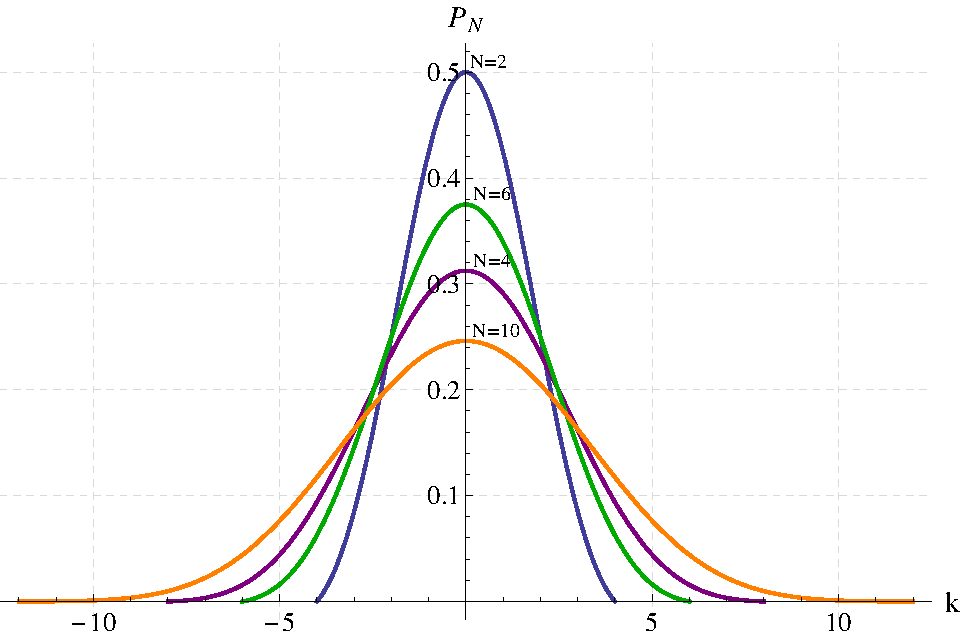
\includegraphics[scale=0.6]{Graphics/ExpectedProbabilityDistribution.pdf}
\caption{A plot showing an envelope of the expected probability distribution over position $x_{k}$
for $N=2,4,6,10$. The probability distributions are the sum of contributions over
all paths.}
\label{fig:ProbabilityDistributionN24610} 
\end{figure}

\begin{figure}[H]
\centering 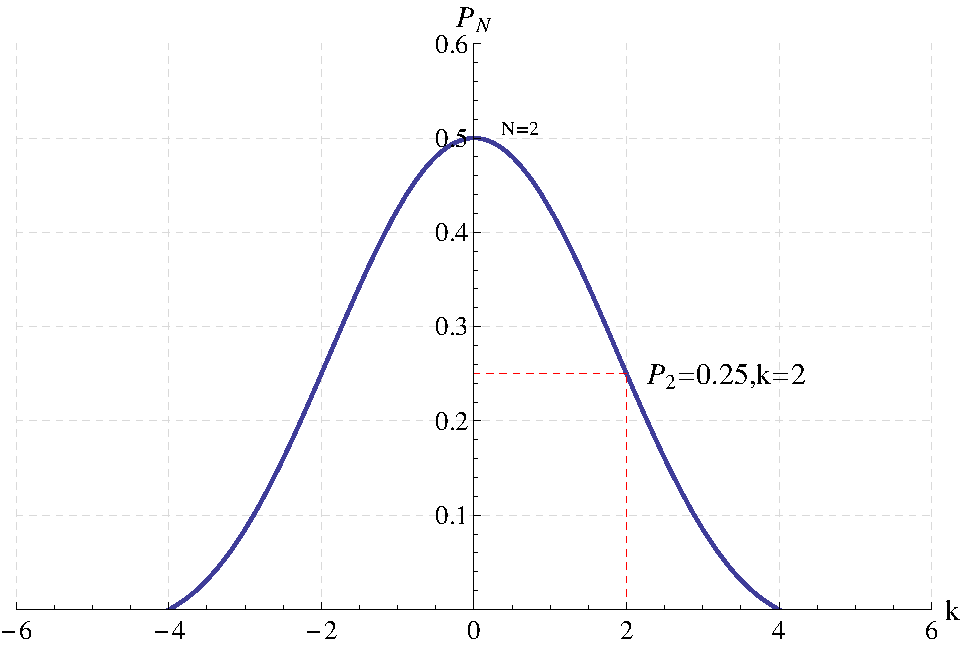
\includegraphics[scale=0.6]{Graphics/ExpectedProbabilityDistributionN2.pdf}
\caption{A plot showing an envelope of the expected probability distribution of displacement $x_{k}$ for $N=2$.
The dashed lines indicate that the end position is twice as likely to be at the origin, $x_{k}=0$ than to be at either $x_{k}=2a$ or $x_{k}=-2a$.}
\label{fig:ProbabilityDistributionN2} 
\end{figure}


\section{Construction of the Partition Function Integral}

In constructing our partition function for an EFJC we will consider a system consisting of $N+1$ particles each of which interacts with its neighbouring particles. The partition function is an integral over phase-space of the exponential of the system's Hamiltonian. The integral represents the sum over all configurations for a $N$-particle system. The Hamiltonian will later allow us to include our desired potential. We work initially in one dimension. The partition function in a system with $N$ links is 
%
\begin{equation}
\mathcal{Z}=\frac{1}{h^{N}}\int\prod_{i=1}^{N}dq_{i}dp_{i}\,\exp\left(-H\left(p_{i},q_{i}\right)/kT\right)\label{ClassicalPartitionFunction}
\end{equation}
%
where $h$ is Planck's constant, $q_{i}$ is the phase space co-ordinate of the $i^{th}$ particle, $p_{i}$ is its momentum, $H\left(p_{i},q_{i}\right)$ is the Hamiltonian, $k$ is the Boltzmann constant, and $T$ is the absolute temperature. The zeroth particle is held static at the origin.

The Hamiltonian, which is a function of both position and momentum, represents the total energy of the system. It is the sum of the kinetic energy and the potential energy of all the constituents,
%
\begin{equation}
\widehat{H}\left(p_{i},q_{i}\right)=\sum_{i=1}^{N}\left(\frac{p_{i}^{2}}{2m}+\Phi\left(q_{i},q_{i-1}\right)\right)\label{Hamiltonian}
\end{equation}
%
where $m$ is the mass of each particle and $\Phi\left(q_{i},q_{i-1}\right)$ is the potential controlling the length of each link. Because the position and momentum parameters are independent in the Hamiltonian it allows us to fully separate the spatial and momentum integrations of the partition function \eqref{ClassicalPartitionFunction}.
%
\begin{align}
\mathcal{Z} & =\frac{1}{h^{N}}\int\prod_{i=1}^{N}dp_{i}\,\exp\left(-\frac{p_{i}^{2}}{2mkT}\right)\,\int\prod_{i=1}^{N}dq_{i}\,\exp\left(-\frac{\sum_{i=1}^{N}\Phi\left(q_{i},q_{i-1}\right)}{kT}\right)\nonumber\\
 & =\frac{1}{h^{N}}Z_{p}Z_{q}\label{SeparableClassicalPartitionFunction}
\end{align}
%
The momentum partition function in \eqref{SeparableClassicalPartitionFunction} is simply a Gaussian integral raised to the power of $N$. This allows us to integrate over the momentum for all the individual links in the chain. It can be simplified to a constant leaving the position partition function integral to be evaluated. 
%
\begin{equation}
Z_{p}=\left(2\pi mkT\right)^{\frac{N}{2}}\label{MomentumPartitionFunction}
\end{equation}
%
The breakdown of the dimensionless partition function gives the position integral $Z_{q}$ a dimension of length to the power of $N$. To simplify the position integral in \eqref{SeparableClassicalPartitionFunction} the potential $\Phi\left(q_{i},q_{i-1}\right)$ needs to be written in terms of a set of variables, $q_{i,i-1}=\left(q_{i}-q_{i-1}\right)$. The Jacobian for this change in variables is unity. A Fourier transform representation of the Dirac delta function is then inserted into the partition function to impose the following constraint. We consider the case where the end-to-end polymer length is equal to $R$, where $R=q_{N}-q_{0}$. We write 
%
\begin{equation}
Z_{q}=\int^{\infty}_{-\infty} \, dR\, Z_{q}\left(R\right)
\end{equation}
%
with
%
\begin{equation}
Z_{q}\left(R\right) = \int\prod_{i=1}^{N}dq_{i} \delta\left(q_{N}-q_{0}-R\right) \exp\left(-\frac{\sum_{i=1}^{N}\Phi\left(q_{i}-q_{i-1} \right)}{kT}\right)
\end{equation}
%
and employ
%
\begin{align}
\delta\left(q_{N}-q_{0}-R\right) & =\delta\left(\sum_{i=1}^{N}q_{i,i-1}-R\right)\nonumber\\
&=\frac{1}{2\pi}\int_{-\infty}^{\infty}d\omega\,\exp\left[i\omega\left(\sum_{i=1}^{N}q_{i,i-1}-R\right)\right]\label{BoundaryCondition}
\end{align}
%
Inserting \eqref{BoundaryCondition} into $Z_{q}\left(R\right)$, we get
%
\begin{align}
Z_{q}\left(R\right) & =\int_{-\infty}^{\infty}\prod_{i=1}^{N}\left[dq_{i,i-1}\exp\left(-\frac{\Phi\left(q_{i,i-1}\right)}{kT}\right)\right]\frac{1}{2\pi}\int_{-\infty}^{\infty}d\omega\,\exp\left[i\omega\left(\sum_{i=1}^{N}q_{i,i-1}-R\right)\right]\nonumber\\
 & =\frac{1}{2\pi}\int_{-\infty}^{\infty}d\omega\,\exp\left(-i\omega R\right)\left[\int_{-\infty}^{\infty}dq_{i,i-1}\,\exp\left(-\frac{\Phi\left(q_{i,i-1}\right)}{kT}\right)\,\exp\left(i\omega q_{i,i-1}\right)\right]^{N}\label{FourierTransformPartitionFunction}
\end{align}
%
Using a suitable potential we can solve \eqref{FourierTransformPartitionFunction} to find the partition function. In the next section we will discuss potential energy functions to describe a FJC and an EFJC.

\subsection{Quadratic Potential}

For an illustration of how one might solve the partition function using the Fourier transform partition function, \eqref{FourierTransformPartitionFunction}, we will begin by fixing the configuration of the EFJC to be linear, and then allow each link to extend harmonically. The focus on a linear configuration takes the model away from a theory of polymers to a theory of an elastic rod. Considering only the 1-D case along the $x$-axis the harmonic
potential is
%
\begin{equation}
\Phi\left(x\right)=\frac{1}{2}\alpha\left(x-a\right)^{2}\label{ElasticPotential}
\end{equation}
%
where $a$ corresponds to the length of each link in the absence of a load, and $\alpha$ is the spring constant. Combining the elastic
potential with \eqref{FourierTransformPartitionFunction} gives
%
\begin{equation}
Z_{q}^{rod}\left(R\right)=\frac{1}{2\pi}\int_{-\infty}^{\infty}d\omega\, \exp\left(-i\omega R\right)\left[\int_{-\infty}^{\infty}dx\, \exp\left(-\frac{\alpha\left(x-a\right)^{2}}{2kT}\right)\, \exp\left(i\omega x\right)\right]^{N}
\end{equation}
%
which when evaluated gives an expression
%
\begin{equation}
Z_{q}\left(R\right)=\left(\frac{2\alpha\pi}{NkT}\right)^{\frac{1}{2}}\left(\frac{2kT\pi}{\alpha}\right)^{\frac{N}{2}}\exp\left(-\frac{\alpha\left(R-aN\right)^{2}}{2kTN}\right)\label{Z_ElasticPotential}
\end{equation}
%
The case described by \eqref{Z_ElasticPotential} corresponds to one configuration of the EFJC with $R=Na$ .
%Since the rod has links that move independently we would expect the maximum partition function value to be at $R=Na$ as there are more configurations the rod can take for end position to be at $R=Na$. The case described by \eqref{Z_ElasticPotential} only takes into account one configuration of the EFJC. 
The results from \figref{GraphElasticPotential} show that \eqref{Z_ElasticPotential} for N=4 describes a Gaussian distribution peaking at $R=4a$. This is the unstretched length of the rod. Irrespective of the many random configurations each link can take within the EFJC, all the links described by this partition function follow the same direction to make the chain comparable to a rod of length $Na$. 

\begin{figure}[htp]
\centering 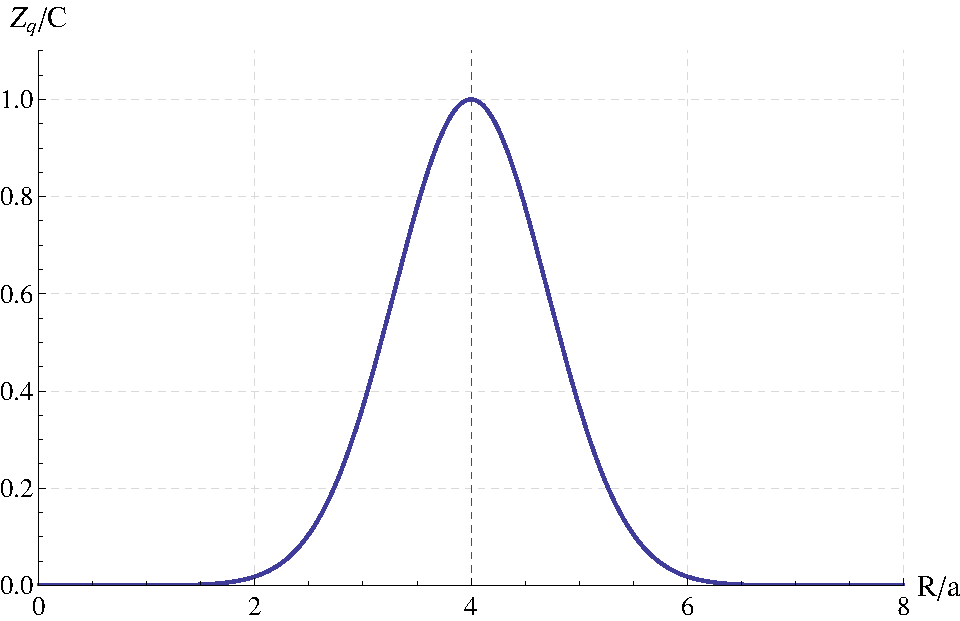
\includegraphics[scale=0.6]{Graphics/zElasticPotential.pdf} 
\caption{A plot showing the value of $Z_{q}/C$ as a function of $R$ using
an harmonic potential for $N=4$. The constant $C$ is a scaling factor and $\alpha/2kTN$ is set to unity.}
\label{fig:GraphElasticPotential} 
\end{figure}

\subsection{Double Potential}

We will begin by looking at how we can create a suitable potential to describe the behaviour of the links that make up the FJC. In modelling each link we will imagine that one end of the link is fixed while the other end is free to lie in any direction characterised by a potential. By subsequently using this method for $N$ links we create an FJC. For example, if the length of a link is $a$, and consider one end of the link to be fixed at a point $\beta$ on the $x$-axis, the other end would be positioned at either $\beta+a$ or $\beta-a$. We can allow each link to have this spatial freedom by setting up a potential, $\Phi\left(x\right)$, that is infinite everywhere except at $a$ and $-a$. The exponential of the potential as seen in \eqref{FourierTransformPartitionFunction}, should correspond to two Dirac delta weighting functions with zero weight everywhere except at $a$ and $-a$. The link cannot be extended further than its unperturbed length, $a$. This potential would describe a non-extendable FJC in one dimension. The potential for the FJC is inserted such that
%
\begin{equation}\label{tophatdeltapotential}
\exp\left(-\frac{\Phi\left(q_{i,i-1}\right)}{kT} \right) = \frac{A}{2}\left( \delta\left(q_{i,i-1}-a\right) + \delta\left(q_{i,i-1}+a\right)  \right)
\end{equation}
%
where $A$ is a constant with dimensions of length. 
%
\begin{figure}[H]
\centering 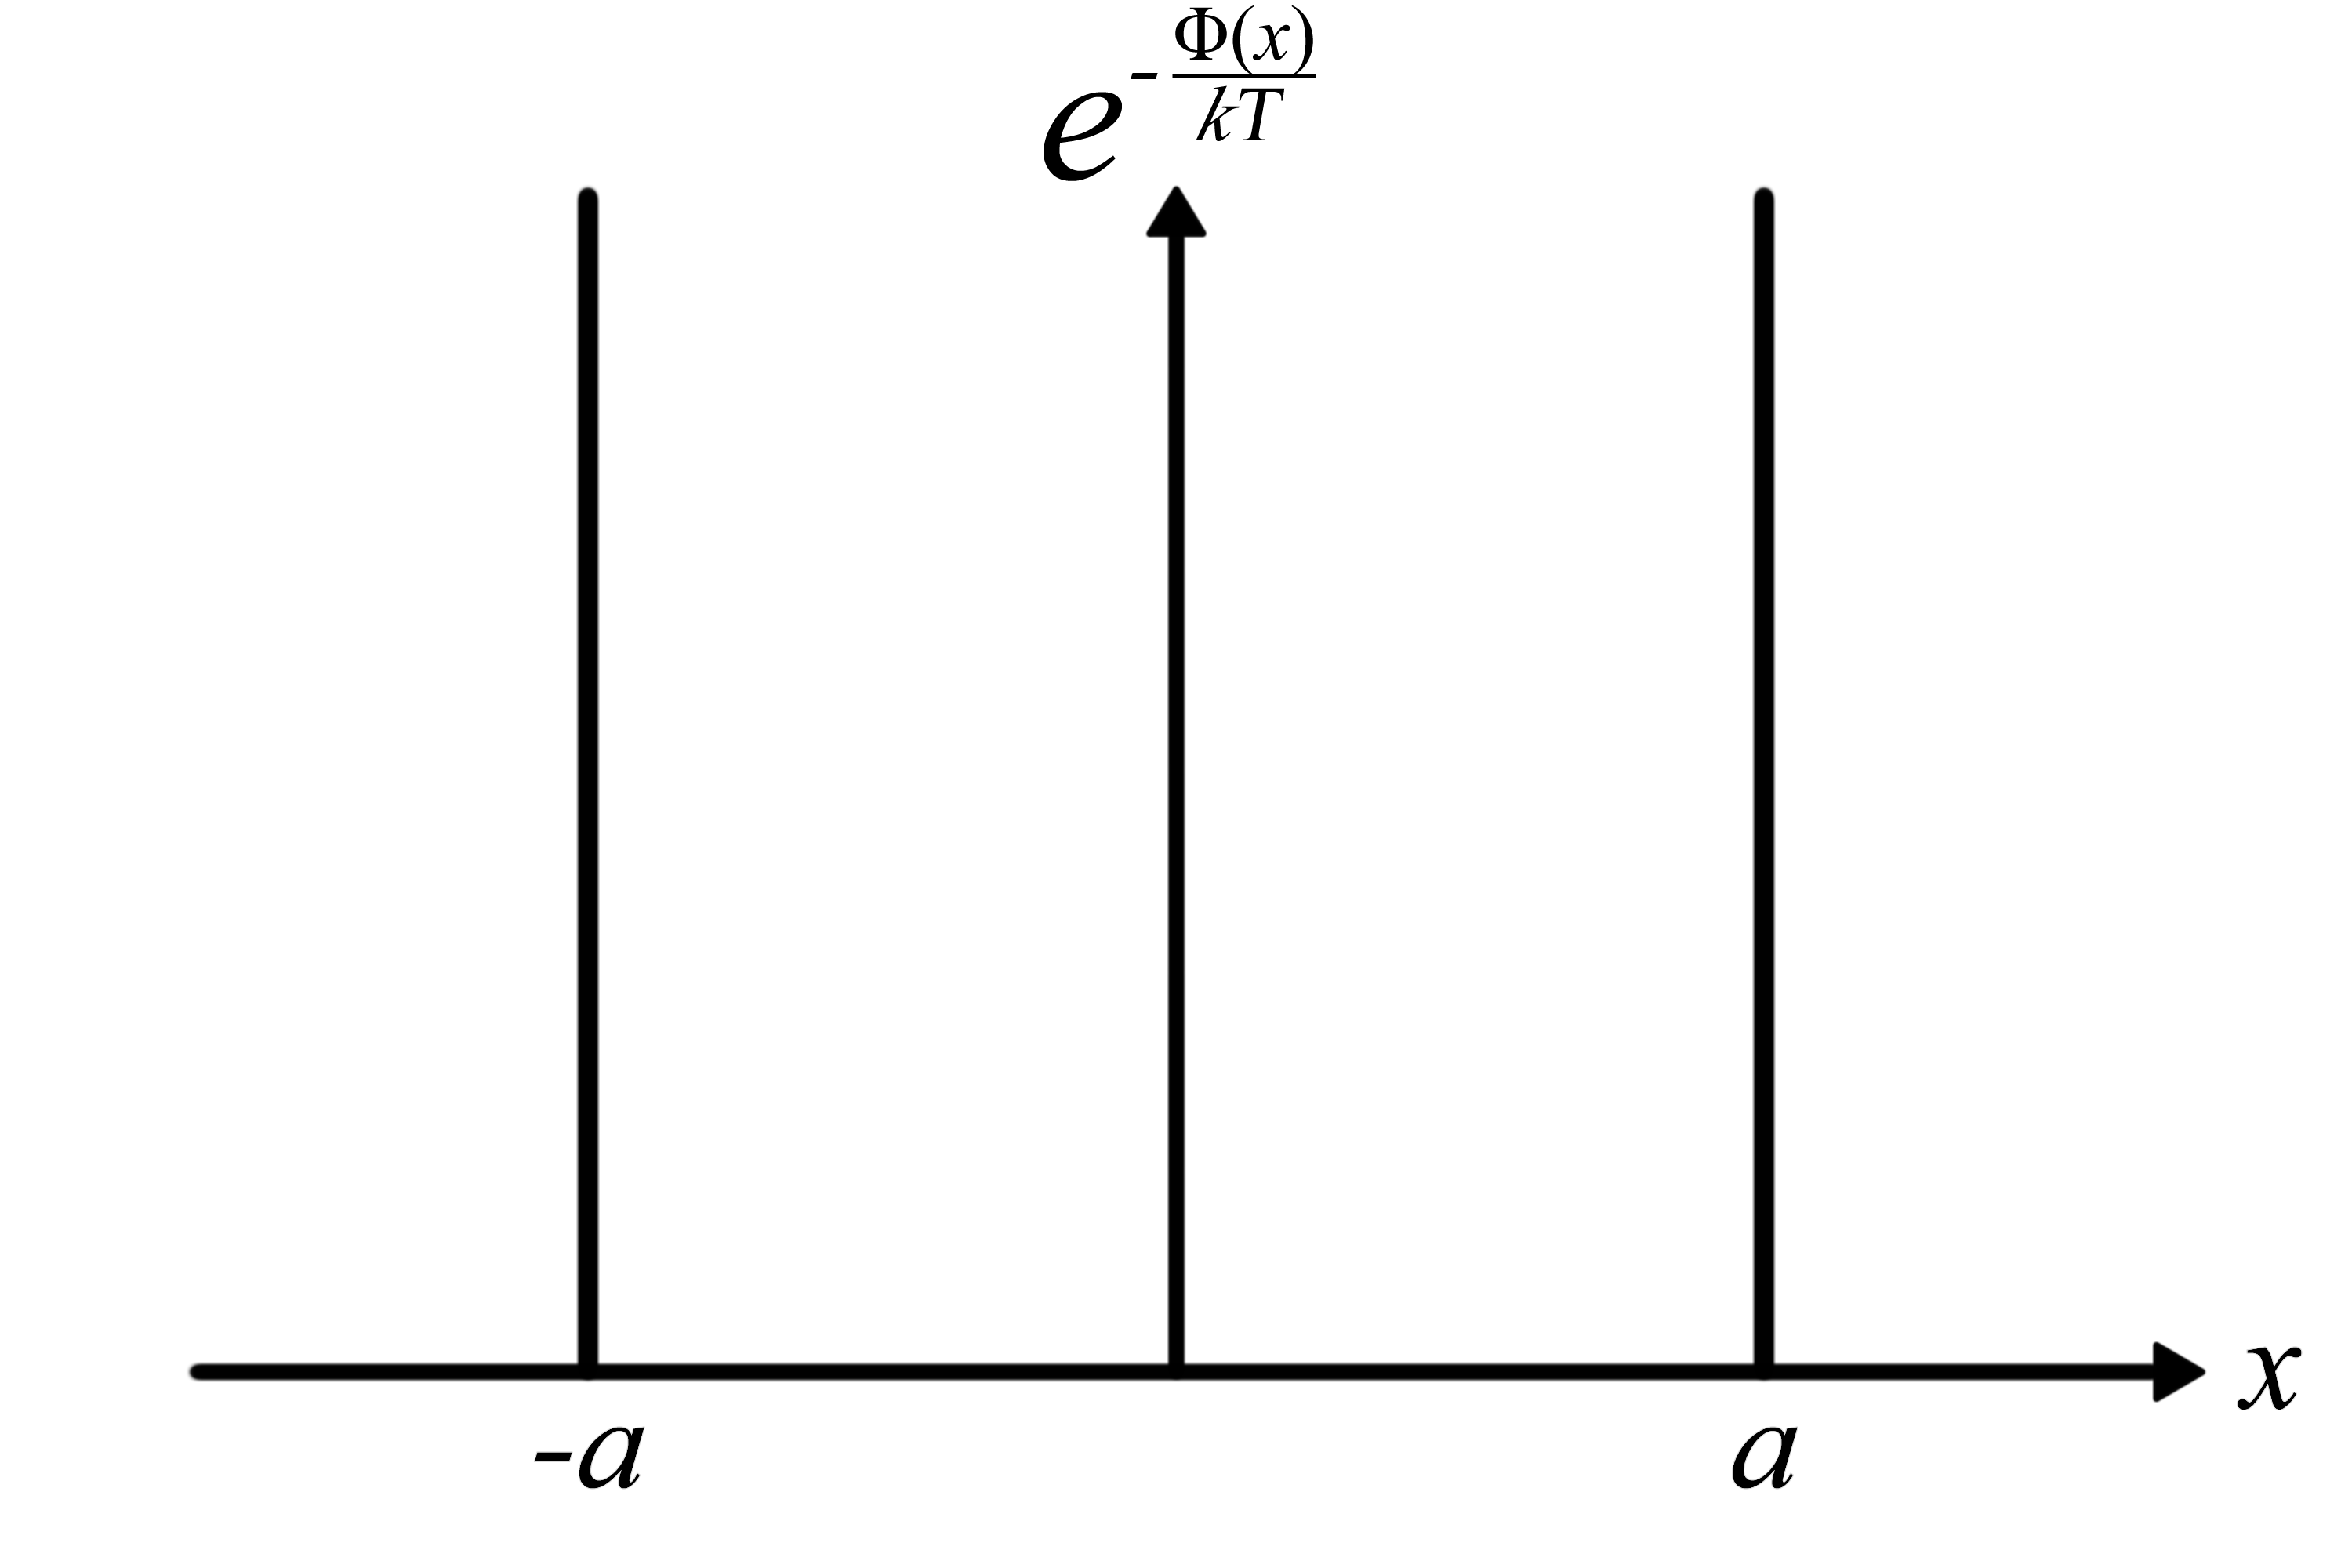
\includegraphics[scale=0.6]{Graphics/DoubleDeltaFunction.png} 
\caption{A plot of the double delta function weighting function where the value of $\exp\left(-\frac{\Phi\left(x\right)}{kT}\right)$ is infinite at $\pm a$.}
\label{fig:DoubleDeltaFunctionPotential} 
\end{figure}
%
The partition function is then
%
\begin{equation}\label{deltapf}
Z_{q}\left(R\right) = \int\prod^{N}_{i=1} dq_{i,i-1}A^{N}\delta\left(\sum_{i=1}^{N}q_{i,i-1} - R\right)\prod_{i=1}^{N}\left( \frac{1}{2}\left( \delta\left(q_{i,i-1}-a \right) + \delta\left(q_{i,i-1}+a \right)   \right)\right)
\end{equation}
%
This is intuitively proportional to a sum over paths, constrained such that the total displacement is $R$ through the first delta function in \eqref{deltapf}. Each step is $\pm a$ imposed by each of the second set of delta functions. It is therefore the sum of all possible outcomes of the symmetric random walk with given $R$. This establishes the analogy between $Z_{q}\left(R\right)$ and $P_{N}\left(R\right)$ derived in \ref{sec:probability}. The normalisation of the probability distribution for $R$ requires that
%
\begin{equation}
P_{N}\left(R \right)= \frac{Z_{q}\left(R\right)}{\int\,dR Z_{q}\left(R\right)}
\end{equation}
%
The transition probability of the analogous random walk is 
%
\begin{equation}
T\left(q_{i,i-1}\right)=  \frac{1}{2}\left( \delta\left(q_{i,i-1}-a \right)+ \delta\left(q_{i,i-1}+a \right)\right)  
\end{equation}
%
This is normalised such that 
%
\begin{equation}
\int^{\infty}_{-\infty}T\left(q_{i,i-1}\right)dq_{i,i-1} = 1
\end{equation}
%
In order to pursue the analogy to a random walk, we need to employ a weighting function such that the transition probability in the analogous random walk is
%
\begin{equation}
T\left(q_{i,i-1}\right)=\frac{\exp \left(-\frac{\Phi\left(q_{i,i-1}\right)}{kT}\right)}{\int^{\infty}_{-\infty} \exp \left( -\frac{\Phi\left(q_{i,i-1}\right)}{kT} \right) dq_{i,i-1}}
\end{equation}
%
which is correctly normalised.


\subsection{Evaluating $\boldsymbol{{Z_{q}\left(R\right)}}$ for the non-extendable Freely Jointed Chain}

Following on from \eqref{deltapf}, where the exponential term is replaced by two delta weighted functions, the partition function
becomes
%
\begin{equation}
Z_{q}\left(R\right)=\frac{A^{N}}{2\pi}\int_{-\infty}^{\infty}d\omega\, e^{-i\omega R}\left[\frac{1}{2}\int_{-\infty}^{\infty}dx\,\left\{ \delta\left(x-a\right)+\delta\left(x+a\right)\right\} e^{i\omega x}\right]^{N}
\end{equation}
%
Taking the terms that correspond to the Fourier transform of the weighting function as $\kappa\left(\omega\right)$, and using the sifting property of the Dirac delta function we get the following \cite{Riley2002},
%
\begin{equation}
Z_{q}\left(R\right)=\frac{A^{N}}{2\pi}\int_{-\infty}^{\infty}d\,\omega e^{-i\omega R}\left[\kappa\left(\omega\right)\right]^{N}
\end{equation}
%
where
%
\begin{align}
\kappa\left(\omega\right)&=\frac{1}{2}\int_{-\infty}^{\infty}\delta\left(x-a\right)e^{i\omega x}dx+\frac{1}{2}\int_{-\infty}^{\infty}\delta\left(x+a\right)e^{i\omega x}dx \\
&=\frac{e^{i\omega a}+e^{-i\omega a}}{2}\\
&=\cos \omega a
\end{align}
%
The partition function then becomes
%
\begin{equation}
Z_{q}\left(R\right)=\frac{A^{N}}{2\pi}\int_{-\infty}^{\infty}d\omega\, e^{-i\omega R}\cos^{N}\omega a
\end{equation}
%
The cos term which is raised to the $N^{th}$ power can be expressed as a sum of exponentials using the binomial theorem,
%
\begin{equation}
\cos^{N}x=\frac{1}{2^{N}}\sum_{k=0}^{N}\binom{N}{k}e^{ix(N-2k)}\label{Cos_Series}
\end{equation}
%
for all integer $k$. Combining this and the general integral representation of the Dirac delta function \cite{Riley2002}
%
\begin{equation}
\delta(x)=\frac{1}{2\pi}\int_{-\infty}^{\infty}e^{-ixt}\, dt
\end{equation}
%
we get
%
\begin{align}
Z_{q}\left(R\right) & =\frac{A^{N}}{2^{N+1}\pi}\sum_{k=0}^{N}\binom{N}{k}\int_{-\infty}^{\infty}e^{-i\omega\left(R+2k-N\right)}\, d\omega\\
 & =\frac{A^{N}}{2^{N+1}\pi}\sum_{k=0}^{N}\binom{N}{k}\delta\left(R+2k-N\right)\label{pfSolved1D_1}\end{align}
%
Here we obtain the partition function for a FJC in one dimension. Evaluating the integral of \eqref{pfSolved1D_1} with respect to $R$ we can show that
%
\begin{equation}
\int Z_{q}\left(R\right)\,dR = \frac{A^{N}}{2^{N+1}\pi}\sum_{k=0}^{N}\binom{N}{k}= \frac{A^{N}}{2\pi} 
\end{equation}
%
and hence
%
\begin{equation}
P_{N}\left(R\right) = \frac{Z_{q}\left(R\right)}{\int Z_{q}\left(R\right)\,dR} = \frac{1}{2^{N}}\sum^{N}_{k=0}\binom{N}{k}\delta(R+2k-N)
\end{equation}
%
as derived earlier in \eqref{pdist}. Taking this further, the partition function for the EFJC will next be calculated using an appropriate weighting function.

\section{Extendable Freely Jointed Chain Model in One Dimension}

\subsection{Potential for an Extendable Freely Jointed Chain}

To make the FJC extendable we replace the double delta function weighting factors with two top-hat functions of finite width $p$. This corresponds to a pair of infinite square wells and since they have a finite width $p$, it allows each link is able to extend and contract by a length $\frac{p}{2}$ without a cost in energy. The normalised transition probability for the random walk analogous to the EFJC would be $T\left(q_{i},q_{i-1}\right)$ such that
%
\begin{equation}
\int^{\infty}_{-\infty}T\left(q_{i,i-1}\right)dq_{i,i-1}=\frac{1}{2p}\left[\int_{-a-\frac{p}{2}}^{-a+\frac{p}{2}}\,dq_{i,i-1} + \int_{a-\frac{p}{2}}^{a+\frac{p}{2}}\,dq_{i,i-1}\right]=1
\end{equation} 
%
The effect of taking the limit of $p\rightarrow0$ whilst preserving the normalisation makes the height of each weighting function infinitely large such that they become delta functions. Analytically, we can show that our top-hat weighting functions become proportional to delta functions in the limit of $p\rightarrow0$ by using a combination of Heaviside functions to express an integral over finite limits as an integral over all space.
%
\begin{equation}
H(x)=\int_{-\infty}^{x}\delta(t)dt\label{HeavisideFunction}
\end{equation}
%
Starting with the top-hat weighting functions in one dimension we can express the weight of the potential as two separate integrals where the width of weighting function $\varsigma(x)$ is contained in the integral limits.
%
\begin{equation}
\int_{a-\frac{p}{2}}^{a+\frac{p}{2}}\varsigma(x)\, dx+\int_{-a-\frac{p}{2}}^{-a+\frac{p}{2}}\varsigma(x)\, dx\label{IntegralOfWeight}
\end{equation}
%
Representing a top-hat weighting function with two Heaviside step functions we have \cite{Bronshtein2007},
%
\begin{equation}
\sqcap\left(x;p\right)\equiv H\left(x+\frac{p}{2}\right)-H\left(x-\frac{p}{2}\right)\label{Top-Hat}
\end{equation}
%
Where $x$ would be the centre position of the top-hat function. The weighting factor in the integrand, and implicitly the potential $\Phi$, will be written 
%
\begin{equation}\label{tophatpotential}
\exp\left(-\frac{\Phi\left(q_{i,i-1}\right)}{kT}\right)= \frac{A}{2p}\left(\sqcap\left(x-a;p\right)+\sqcap\left(x+a;p\right)\right)
\end{equation}
%
Where $A$ again has dimensions of length, and will turn out to be analogous to the $A$ in \eqref{tophatdeltapotential}. Using \eqref{Top-Hat} each integral in \eqref{IntegralOfWeight} can now be expressed as an integral over all space,
%
\begin{align}
\int_{a-\frac{p}{2}}^{a+\frac{p}{2}}\varsigma(x)\, dx & =\int_{-\infty}^{\infty}\sqcap\left(x-a;p\right)\varsigma(x)\, dx\\
\int_{-a-\frac{p}{2}}^{-a+\frac{p}{2}}\varsigma(x)\, dx & =\int_{-\infty}^{\infty}\sqcap\left(x+a;p\right)\varsigma(x)\, dx
\end{align}
%
The positions $a$ and $-a$ correspond to the positions of the top-hat potentials as shown in \figref{DoubleTophatPotential}. Since the value of $p$ is small and finite we can use the mean value theorem for integration to express each integral as,
%
\begin{align}
\int_{-\infty}^{\infty}\frac{1}{p}\sqcap\left(x-a;p\right)\varsigma(x)\, dx & =\varsigma\left(\tau\right)\\
\int_{-\infty}^{\infty}\frac{1}{p}\sqcap\left(x+a;p\right)\varsigma(x)\, dx & =\varsigma\left(\tau'\right)
\end{align}
%
for $\tau$ such that $x-a-\frac{p}{2}\leq\tau\leq x-a+\frac{p}{2}$ and $\tau'$ such that $x+a-\frac{p}{2}\leq\tau'\leq x+a+\frac{p}{2}$. Then taking the limit of $p\rightarrow0$ we get,
%
\begin{align}
\lim_{p\to0}\left[\int_{-\infty}^{\infty}\frac{1}{p}\sqcap\left(x-a;p\right)\varsigma(x)\, dx\right] & =\lim_{p\to0}\left[\varsigma\left(x-a\pm\frac{p}{2}\right)\right] = \varsigma\left(x-a\right)\\
\lim_{p\to0}\left[\int_{-\infty}^{\infty}\frac{1}{p}\sqcap\left(x+a;p\right)\varsigma(x)\, dx\right] & =\lim_{p\to0}\left[\varsigma\left(x+a\pm\frac{p}{2}\right)\right] = \varsigma\left(x-a\right)
\end{align}
%
Thus in the $p \rightarrow 0$ limit this procedure gives rise to two delta functions at the positions $a$
and $-a$,
%
\begin{align}
\lim_{p\to0}\left[\frac{1}{p}\sqcap\left(x-a;p\right)\right] & =\delta\left(x-a\right)\\
\lim_{p\to0}\left[\frac{1}{p}\sqcap\left(x+a;p\right)\right] & =\delta\left(x+a\right)
\end{align}
%
The analysis demonstrates that the top-hat potentials reduce to delta functions in the limit of $p\rightarrow0$ which we would expect. Moreover, by applying the appropriate $p\rightarrow0$ limits in the final expression for $Z_{q}\left(R\right)$ for an EFJC, we can check that it behaves like a non-extendable FJC. In other words, \eqref{tophatpotential} should tend towards \eqref{tophatdeltapotential}.
%
\begin{figure}[htp]
 \centering 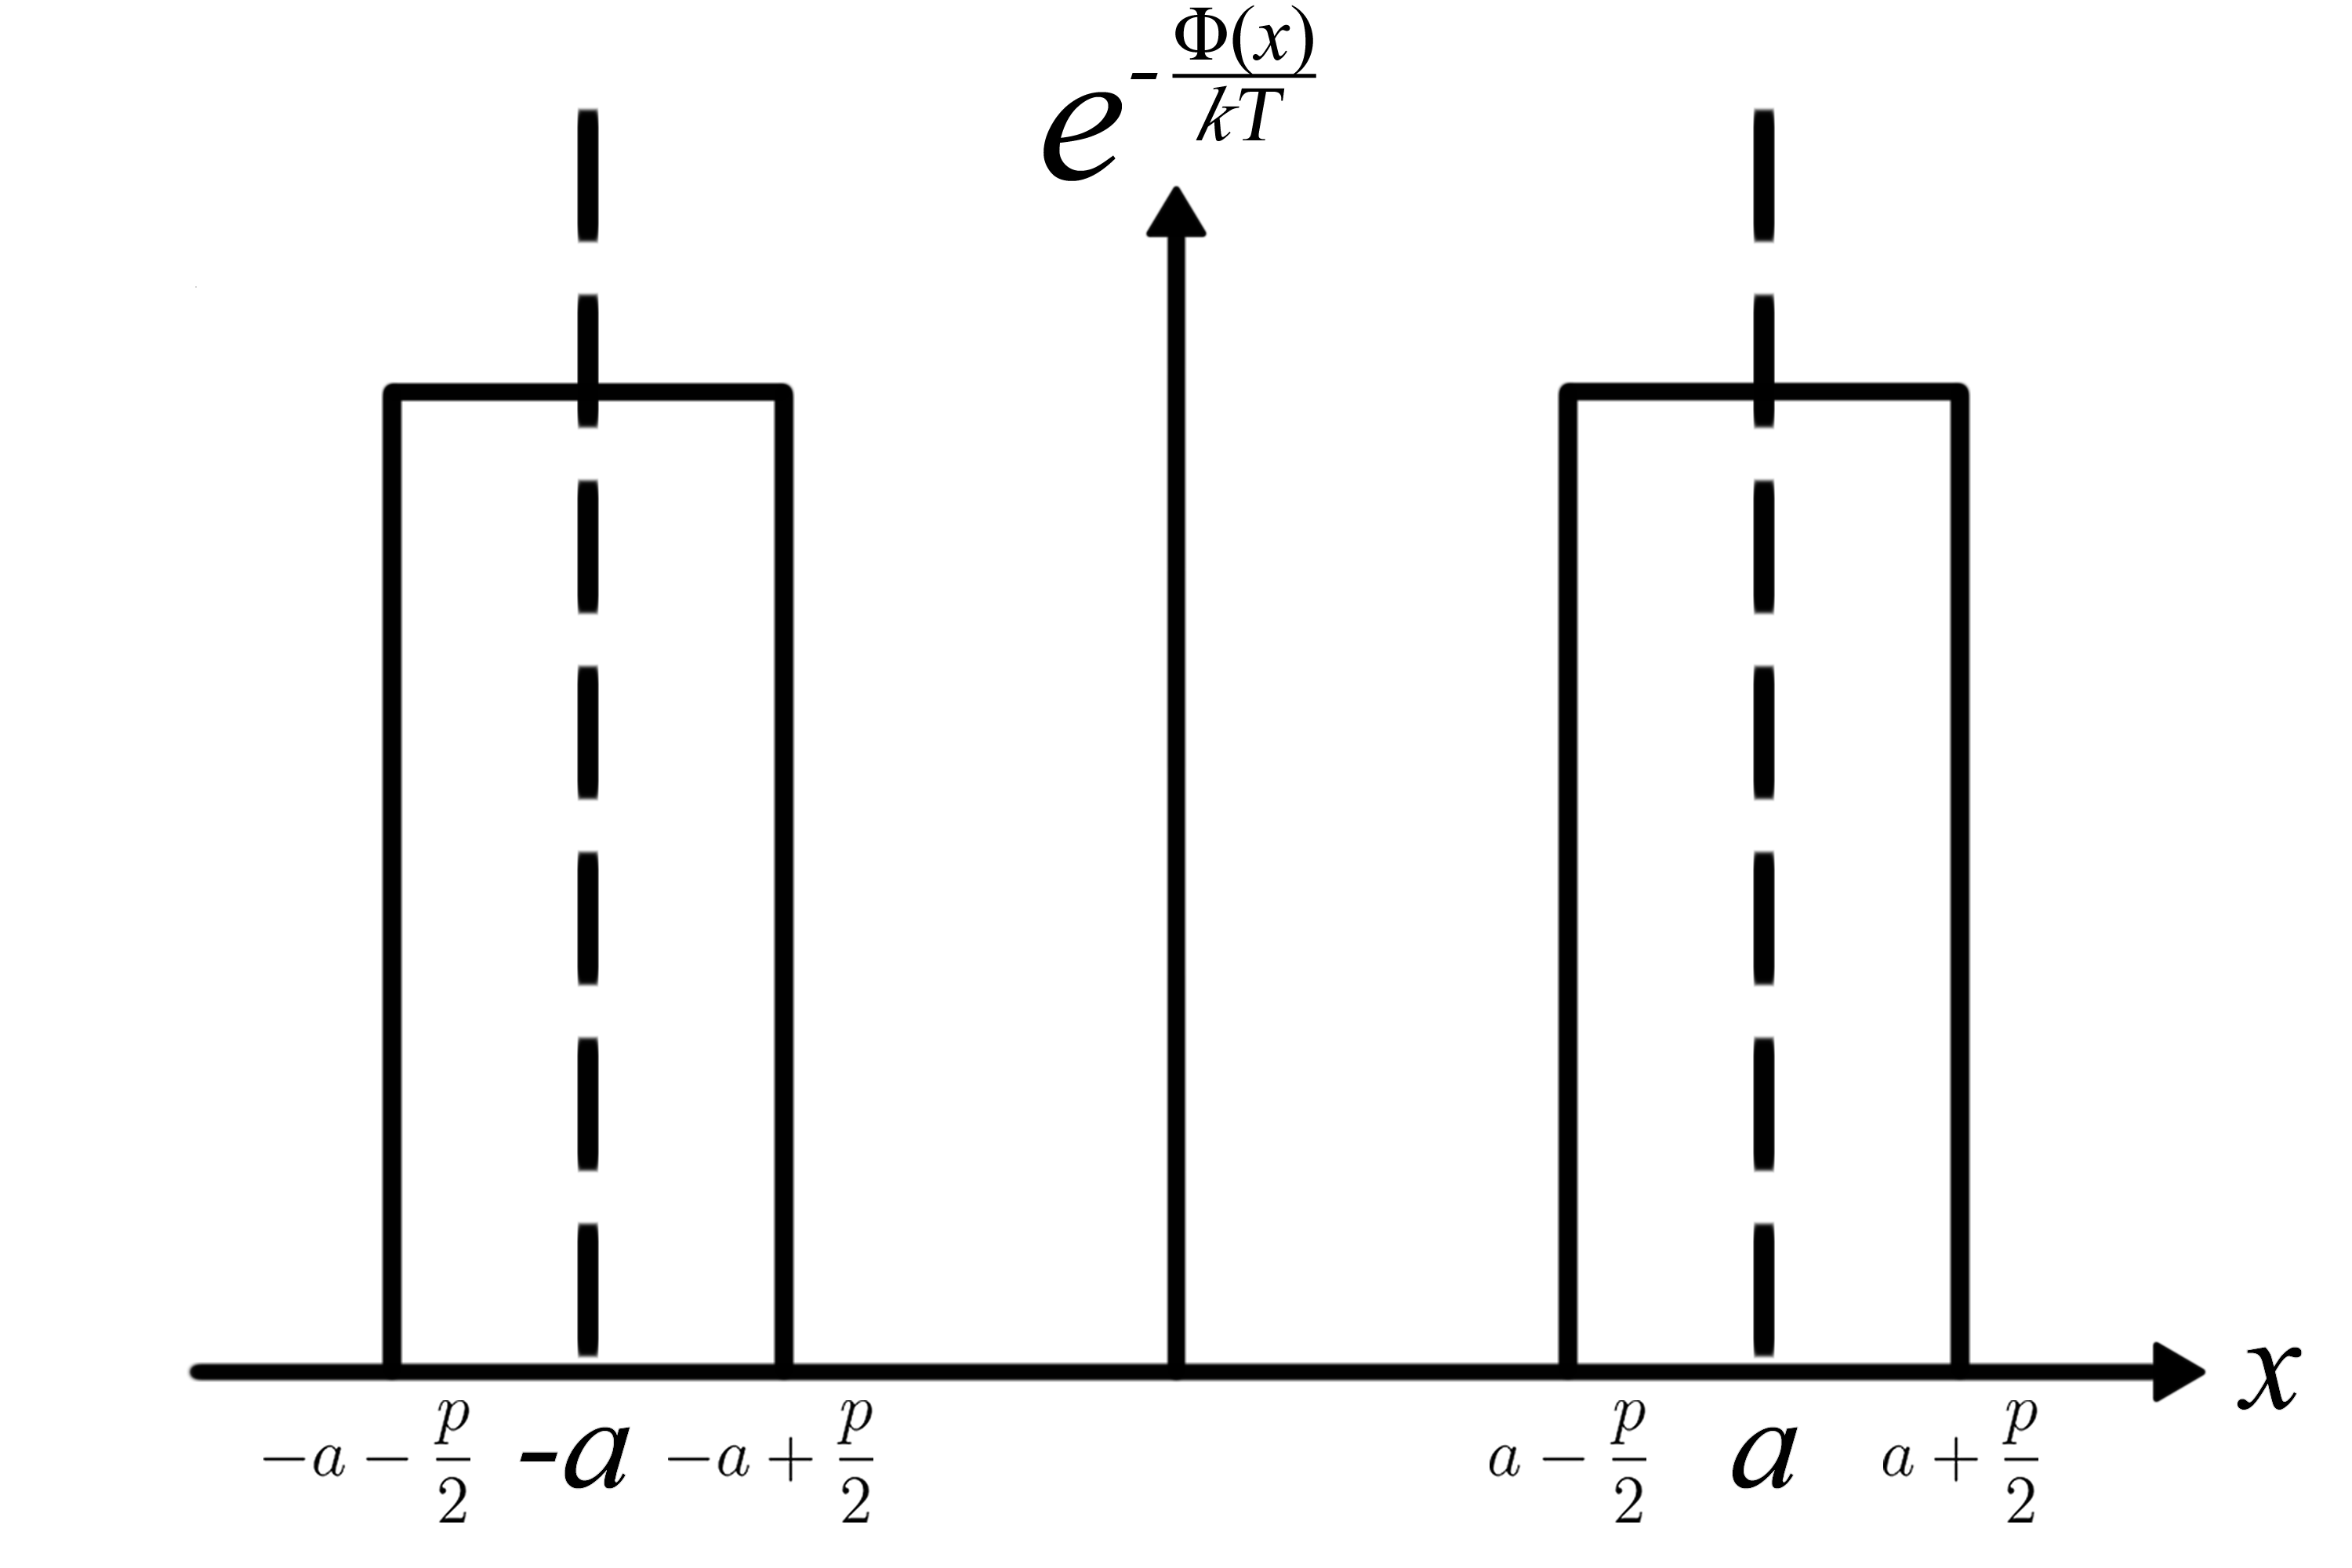
\includegraphics[scale=0.6]{Graphics/DoubleTopHatFunction.png} 
\caption{A plot showing a pair of top-hat functions as the weighting function with
a finite thickness $p$ and finite height. The top-hats are centred about $a$ and $-a$.}
\label{fig:DoubleTophatPotential} 
\end{figure}

\subsection{Extendable Freely Jointed Chain}

Working from \eqref{FourierTransformPartitionFunction} taking our one dimensional model along the $x$-axis in a Cartesian co-ordinate system we have,
%
\begin{equation}
Z_{q}\left(R\right)=\frac{1}{2\pi}\int_{-\infty}^{\infty}d\omega\, e^{-i\omega R}\left[\int_{-\infty}^{\infty}d\Delta x\, e^{-\frac{\Phi\left(\Delta x\right)}{kT}}\, e^{i\omega\Delta x}\right]^{N}\label{FourierTransFormPartitionFunction1D}
\end{equation}
%
We have already obtained the partition function for the FJC by replacing the weighting factor in the integrand with a sum of two delta functions. For a EFJC we will now use two top-hat functions as the weighting factor for the potential, the Fourier transform weighted potential, $G\left(\omega\right)$, is then written as two integrals over finite limits. The Fourier transform of the weighting factor for the EFJC becomes,
%
\begin{align}
G\left(\omega\right) & =\int_{-\infty}^{\infty}\, e^{-\frac{\Phi\left(\Delta x\right)}{kT}}\, e^{i\omega\Delta x}d\Delta x\label{FTWP}\\
 & =\frac{A}{2p}\int_{-a-\frac{p}{2}}^{-a+\frac{p}{2}}e^{i\omega\Delta x}\, d\Delta x+\frac{A}{2p}\int_{a-\frac{p}{2}}^{a+\frac{p}{2}}e^{i\omega\Delta x}\, d\Delta x\\
 & =\left(\frac{2A}{\omega p}\right)\cos\omega a \, \sin \frac{\omega p}{2} \label{FourierTransformWeightedPotential1D}
\end{align}
%
Combining \eqref{FourierTransFormPartitionFunction1D} and \eqref{FourierTransformWeightedPotential1D} gives a simpler expression for the partition function,
%
\begin{equation}
Z_{q}\left(R\right)=\frac{1}{2\pi}\int_{-\infty}^{\infty}d\omega\, e^{-i\omega R}\left[\left(\frac{2A}{\omega p}\right)\cos\omega a\,\sin\frac{\omega p}{2}\right]^{N}\label{PartitionFunctionUnsolved1D}
\end{equation}
%
At this point we can begin to consider how $p$ affects the solution and enquire whether an approximation of small $p$ helps to simplify \eqref{PartitionFunctionUnsolved1D} to produce a neat solution. It is perfectly acceptable to take the small approximation of $p$ since we have stated that the width of the top-hat weighted potential is small and finite. For the EFJC different methods can be used to impose the limit where $p$ becomes finite producing the desired result for $Z_{q}\left(R\right)$. Each method starts from \eqref{PartitionFunctionUnsolved1D}.

\subsection{Imposing the limit of $p$ by the small approximation of $\boldsymbol{\sin\left(\frac{\omega p}{2}\right)}$}

Applying the small approximation of $p$ we linearise the trigonometric function such that $\sin\left(\frac{\omega p}{2}\right)\simeq\frac{\omega p}{2}$ before the integral is evaluated. \eqref{PartitionFunctionUnsolved1D}
becomes,
%
\begin{equation}
Z_{q}\left(R\right)=\frac{A^{N}}{2\pi}\int_{-\infty}^{\infty}e^{-i\omega R}\cos^{N}\omega a\, d\omega\label{pfSmallLimitP}
\end{equation}
%
Then using \eqref{Cos_Series} and the integral representation of the Dirac delta function we recover the partition function for the FJC,
%
\begin{equation}
Z_{q}\left(R\right)=\frac{A^{N}}{2^{N+1}\pi}\sum_{k=0}^{N}\binom{N}{k}\delta\left(R+2k-N\right)
\end{equation}
%
With the small approximation of $p$, we have effectively approximated $G\left(\omega\right)$ to first order which gives the model for a FJC. Next we will include the higher order terms in the expansion
of $\sin\left(\frac{\omega p}{2}\right)$.

\subsection{Using the Taylor expansion of $\sin \frac{\omega p}{2}$ to include higher order terms}

By employing the expansion of $\sin(\frac{\omega p}{2})$ we are including higher order terms in the calculation of $Z_{q}$ before imposing the limit of $p\rightarrow0$. Working from \eqref{PartitionFunctionUnsolved1D} we can write $\cos^{N} \omega a$ as a series of exponentials using \eqref{Cos_Series}. The Taylor expansion of the sine term can be written as
%
\begin{equation}\label{sin_taylor}
\frac{ \sin^{N} \left(\frac{\omega p}{2}\right)}{\left(\frac{\omega p}{2}\right)^{N}} =  \sum_{m=0}^{\infty}A_{m}\left(\omega p \right)^{m}
\end{equation}
%
The partition function for an EFJC then becomes
%
\begin{equation}
Z_{q}\left(R\right)=\frac{A^{N}}{2^{N+1}\pi}\sum_{k=0}^{N}\binom{N}{k}\int_{-\infty}^{\infty}e^{-i\omega\left(R+2k-N\right)}\sum_{m=0}^{\infty}A_{m}\left(\omega p\right)^{m}\, d\omega
\end{equation}
%
The complex integral maybe be written \cite{Bronshtein2007}
%
\begin{equation}
\int_{-\infty}^{\infty}\omega^{b}e^{-i\alpha\omega}\, d\omega=2\pi i^{b}\delta^{(b)}(\alpha)
\end{equation}
%
where $\delta^{(b)}(\alpha)$ is the $b^{th}$ derivative of the delta function. So inserting this solution into the power series we get
%
\begin{equation}
Z_{q}\left(R\right)=\frac{A^{N}}{2^{N+1}\pi}\sum_{k=0}^{N}\binom{N}{k} \sum^{\infty}_{m=0}A_{m}2\pi (ip)^{m}\delta^{m}\left(\alpha\right)
\end{equation}
%
where $\alpha=R+2k-N$. We can then express the differential of the delta functions as,
$\delta^{n}\left(\gamma\right)=\left(-1\right)^{n}n!\delta\left(\gamma\right)/\gamma^{n}$, so
%
\begin{equation}
Z_{q}\left(R\right)=\frac{A^{N}}{2^{N+1}\pi}\sum_{k=0}^{N}\binom{N}{k} \sum^{\infty}_{m=0}G_{m}p^{m}\delta\left(\alpha\right)
\end{equation}
%
where $G_{m} = A_{m}2\pi \left(-i\right)^{m} m!$. Having the Dirac delta function in the result for $Z_{q}$ is important because it shows that only when $\alpha=0$ do we have a non-zero result for the partition function. At this stage we can take the limit of $p\rightarrow0$,
%
\begin{equation}
Z_{q}\left(R\right)=\frac{A^{N}}{2^{N+1}\pi}\sum_{k=0}^{N}\binom{N}{k}\left(G_{0}\delta\left(\alpha\right) + \lim_{p \to 0}\sum^{\infty}_{m=1}G_{m}p^{m}\delta\left(\alpha\right) \right)
\end{equation}
%
which becomes,
%
\begin{equation}
Z_{q}\left(R\right)=\frac{A^{N}}{2^{N+1}\pi}\sum_{k=0}^{N}\binom{N}{k}G_{0}\delta\left(\alpha\right)\label{pfSolved1D_2}
\end{equation}
%
as required, as in \eqref{pfSolved1D_1}. 

Both methods described above yield the same result for the small approximation for $p$, with the solution being the same as the FJC. However, the analysis is somewhat misleading since the general partition function appears to be a modified set of delta functions, rather than a continuous function of $R$. This outcome is a consequence of assuming that the series in $p$ produces convergent integrals which is unclear. In order to obtain the correct partition function for the EFJC we will need to  consider the exact solution of \eqref{PartitionFunctionUnsolved1D}.

\subsection{Expanding the Fourier Transform of the Potential as a Series}

With the Fourier transform of the weighted potential raised to the $N^{th}$ power we can express the trigonometric functions as a series of exponentials with sum over $k^{'}$ and $k$ using the binomial theorem. The expression for $\cos^{N}\left(x\right)$ is given by \eqref{Cos_Series} and the term for $\sin^{N}\left(x\right)$ is given by,
%
\begin{equation}
\sin^{N}x=\frac{1}{(2i)^{N}}\sum_{k^{'}=0}^{N}\binom{N}{k^{'}}(-1)^{k^{'}}e^{ix(N-2k^{'})}\label{Sin_Series}
\end{equation}
%
Using \eqref{Cos_Series} and \eqref{Sin_Series} for the trigonometric terms, \eqref{PartitionFunctionUnsolved1D} becomes
%
\begin{equation}
Z_{q}\left(R\right)=\frac{A^{N}}{2^{N+1}\pi i^N p^{N}}\sum_{k^{\,}=0}^{N}\sum_{{k}'=0}^{N}\binom{N}{k}\binom{N}{k'}\left(-1\right)^{k^{'}}\int_{-\infty}^{\infty}\frac{e^{i\omega\left(a\left(N-2k\right)+\frac{p}{2}\left(N-2{k}'\right)-R\right)}}{\omega^{N}}\, d\omega\label{pfExactUnsolved1D}
\end{equation}
%
The complex multipole integral takes the form,
%
\begin{equation}
\int_{-\infty}^{\infty}\frac{e^{i\omega\zeta}}{\omega^{N}}\, d\omega\,=\frac{\pi i^{N}\zeta^{N-1}}{\left(N-1\right)!}\sgn\left(\zeta\right)\label{MultipoleIntegral}
\end{equation}
%
where
%
\begin{equation}
\sgn\left(\zeta\right)=\begin{cases}
-1 & \text{ for }\zeta<0\\
0 & \text{ for }\zeta=0\\
1 & \text{ for }\zeta>0\end{cases}\label{sign}
\end{equation}
%
Using \eqref{MultipoleIntegral} to evaluate the integral, \eqref{pfExactUnsolved1D} becomes
%
\begin{equation}
Z_{q}\left(R\right)=\frac{A^{N}}{2^{N+1} p^{N}}\sum_{k^{\,}=0}^{N}\sum_{{k}'=0}^{N}\binom{N}{k}\binom{N}{k'}\left(-1\right)^{k^{'}}\frac{\eta^{N-1}}{\left(N-1\right)!}\sgn\left(\eta\right)\label{PartitionFunction1DSolved}
\end{equation}
%
where $\eta=a\left(N-2k\right)+\frac{p}{2}\left(N-2{k}'\right)-R$.

Referring to the case where $N=2$, we see in \figref{1DN2Orig} that the partition function given by \eqref{PartitionFunction1DSolved} is twice as large at $R=0$ than at $R=2$. This is what we expect to find for the FJC chain in 1D. For the case when $N=1$ only one link exists in the FJC which means that the end point can only lie at one of the two positions denoted by $R=1,-1$. A plot of $Z_{q}\left(R\right)$ where $N=1$ and $p=0.1a$ is shown in \figref{1DN1Orig}. For the cases where $N$ is an odd number the partition function at an even position, $k=0,2,4,6,8,..$, will always be zero since the end of the EFJC will never reach those positions unless $p$ is larger.

As the number of links increases in the EFJC we see from \figref{1DN8Orig} and \figref{1DN10Orig} that \eqref{PartitionFunction1DSolved} begins to break down giving irregular results. The nature of this problem is due to the fact that as $N$ gets larger the cancellations due to $\sgn(\eta)$ in the polynomials become extremely delicate. The sums in $Z_{q}\left(R\right)$ for low $N$ involves relevant cancellations to give the required result, as shown in Table. \ref{table:kernal}.

To overcome this problem we can impose constraints from the analysis of \eqref{PartitionFunction1DSolved} to assist with the cancellations that take place. In the polynomial $\eta^{N-1}\sgn\left(\eta\right)$ we will rewrite $\eta$ such that,
%
\begin{equation}\label{eta1}
\eta=F(k,k')-R\end{equation}
%
Where
%
\begin{equation}
F(k,k')=a(N-2k)+\frac{p}{2}(N-2k')\label{Adjustment1}
\end{equation}
%
To impose the correct constraints let us examine in detail the nature of \eqref{PartitionFunction1DSolved}. The partition function is a sum of terms labelled by $k$ and $k'$. We shall refer to $k$ as an index denoting the coarse scale structure of $Z_{q}(R)$ and $k'$ as a label of the fine scale structure for reasons that will become clear later. For a given value of $k$, the core of the expression is
%
\begin{equation}\label{eta2}
\sum_{k'=0}^{N}\left(-1\right)^{k'}\eta^{N-1}\sgn (\eta)
\end{equation}
%
From \eqref{eta1} and \eqref{eta2} we can deduce that for $R < \min_{k'}(F(k,k')) = F(k,N) = a(N-2k)-\frac{Np}{2}$, $\eta > 0$ for all $k'$. Therefore $\sgn\left(\eta\right) = 1$. Hence for $R$ below such a threshold, the core expression reduces to
%
\begin{equation}\label{eta3}
\sum_{k'=0}^{N}\left(-1\right)^{k'}\eta^{N-1}
\end{equation}
%
By writing $\eta$ as $A+Bk'$, the evaluation of \eqref{eta3} requires us to consider
%
\begin{equation}
\sum^{N}_{k'=0}\binom{N}{k'}\left(-1\right)^{k'}k'^{m} 
\end{equation} 
%
with $m$ taking integer values between zero and $N-1$. However, it may be shown that all such summations are zero, for $m < N$. Similarly, for $R> \max_{k'}(F(k,k'))=F(k,0)=a(N-2k)+\frac{Np}{2}$ we find that $\eta<0$ and $\sgn(\eta)=-1$ for all $k'$. Once again the core expression reduces to
%
\begin{equation}
\sum^{N}_{k'=0}\binom{N}{k'}\left(-1\right)^{k'}\eta^{N-1}
\end{equation}
%
and by similar reasoning, this vanishes.

We find, therefore, that contributions to $Z_{q}\left(R\right)$ for a given $k$ in \eqref{PartitionFunction1DSolved} only arise for the region $a(N-2k)-\frac{Np}{2}\leq R \leq a(N-2k)+\frac{Np}{2}$. This corresponds to a region of width $Np$ about a central position $a(N-2k)$. Within this range, a non-zero contribution to $Z_{q}\left(R\right)$ is made from the sum over $k'$, with modulation due to the change in sign of $\eta$ at some point in the sum over $k'$.

Thus each value of $k$ in the expression for $Z_{q}\left(R\right)$ defines a coarse region of $R$ within which non-zero contributions are made due to the summation over $k'$. For this reason we characterise $k$ as the coarse structure label and $k'$ as a fine structure label.

Returning to \eqref{eta2}, we see that it is a sum of polynomials in $R$, of order $N-1$, each with a different zero corresponding to $R=F(k,k')$. For values of $R$  further and further away from each zero, the polynomial $(F(k,k')-R)^{N-1}$ increases rapidly, especially for large $N$ and yet the sum of all the terms vanishes. This is due to a very delicate cancellations of terms. In numerical implementations, such a cancellation will fail in detail, as is shown by the breakdown in the calculation of $Z_{q}\left(R\right)$ for larger $N$ in \figref{1DN8Orig} and \figref{1DN10Orig}. This difficulty, however, may be removed if we help the core expression to vanish for $R$ outside the coarse scale range of values. We multiply it by a top hat function which is zero outside the range $a(N-2k) -\frac{Np}{2} < R < a(N-2k)+\frac{Np}{2}$ and unity within. This function is 
%
\begin{equation}
\Theta(R,k)=H(R-F(k,N))H(F(k,0)-R)\label{AdjustmentTopHat}
\end{equation}
%
and hence the expression for $Z_{q}(R)$ may be revised to,
%
\begin{equation}
Z_{q}\left(R\right)=\frac{A^{N}}{2^{N+1} p^{N}}\sum_{k^{\,}=0}^{N}\sum_{{k}'=0}^{N}\binom{N}{k}\binom{N}{k'}\left(-1\right)^{k^{'}}\frac{\eta^{N-1}}{\left(N-1\right)!}\sgn\left(\eta\right)\Theta(R,k)\label{NewPartitionFunction1DSolved}
\end{equation}
%
A plot of the partition function using \eqref{NewPartitionFunction1DSolved} can be seen in \figref{Z1D}. For the specific cases where $N=8$ and $N=10$ we can see that \figref{1DN8} and \figref{1DN10} show stable results. A detailed breakdown of the modified partition function for $N=2$ is shown in Table. \ref{table:mod_kernal}.

\renewcommand{\arraystretch}{1.5}
\begin{table}[h]
\centering
    \begin{tabular}{ c c c } \hline
    $R$ & $\binom{N}{k}\binom{N}{k'}\left(-1\right)^{k^{'}}\frac{\eta^{N-1}}{\left(N-1\right)!}\sgn\left(\eta\right)$ & $\sum_{k,k'}^{N}\binom{N}{k}\binom{N}{k'}\left(-1\right)^{k^{'}}\frac{\eta^{N-1}}{\left(N-1\right)!}\sgn\left(\eta\right)$ \\ [1ex] \hline\hline 
    -2  & \{4.2,\,-8,\,3.8,\,4.4,\,-8,\,3.6\},\,0.2,\,0,\,0.2  & 0.4 \\ 
    -1  & \{3.2,\,-6,\,2.8,\,2.4,\,-4,\,1.6,\,0.8,\,-2,\,1.2\} & 0   \\ 
    0   & \{2.2,\,-4,\,1.8\},\,0.4,\,0,\,0.4,\,\{1.8,\,-4,\,2.2\}  & 0.8 \\ 
    1   & \{1.2,\,-2,\,0.8,\,1.6,\,-4,\,2.4,\,2.8,\,-6,\,3.2\} & 0   \\ 
    2   & 0.2,\,0,\,0.2,\,\{3.6,\,-8,\,4.4,\,3.8,\,-8,\,4.2\}  & 0.4 \\ [1ex] \hline
    \end{tabular}
\caption{A breakdown of the partition function \eqref{PartitionFunction1DSolved} for N=2. The relevant summations in the curly brackets are the cancellations that occur in the partition to give a desired result. For small $N$ these cancellations are simple which become more difficult for larger $N$. This is seen in \figref{1DN10Orig}.}
\label{table:kernal}
\end{table}

\begin{table}[h]
\centering
    \begin{tabular}{ c c c } \hline
    $R$ & $\binom{N}{k}\binom{N}{k'}\left(-1\right)^{k^{'}}\frac{\eta^{N-1}}{\left(N-1\right)!}\sgn\left(\eta\right)\Theta(R,k)$ & $\sum_{k,k'}^{N}\binom{N}{k}\binom{N}{k'}\left(-1\right)^{k^{'}}\frac{\eta^{N-1}}{\left(N-1\right)!}\sgn\left(\eta\right)\Theta(R,k)$ \\ [1ex] \hline\hline 
    -2  & \{0,\,0,\,0,\,0,\,0,\,0\},\,0.2,\,0,\,0.2  & 0.4 \\ 
    -1  & \{0,\,0,\,0,\,0,\,0,\,0,\,0,\,0,\,0\} & 0   \\ 
    0   & \{0,\,0,\,0\},\,0.4,\,0,\,0.4,\,\{0,\,0,\,0\}  & 0.8 \\ 
    1   & \{0,\,0,\,0,\,0,\,0,\,0,\,0,\,0,\,0\} & 0   \\ 
    2   & 0.2,\,0,\,0.2,\,\{0,\,0,\,0,\,0,\,0,\,0\}  & 0.4 \\ [1ex] \hline
    \end{tabular}
\caption{A breakdown of the modified partition function \eqref{NewPartitionFunction1DSolved} for N=2. The values that contributed to the cancellations in the partition function \eqref{PartitionFunction1DSolved} have been set to zero by the function $\Theta$. Only values that contribute to the overall partition function are included in the summations. This works for all N.}
\label{table:mod_kernal}
\end{table}


\begin{figure}[htp]
\centering
\begin{tabular}{cc}
\subfloat[N=1]{\label{fig:1DN1Orig}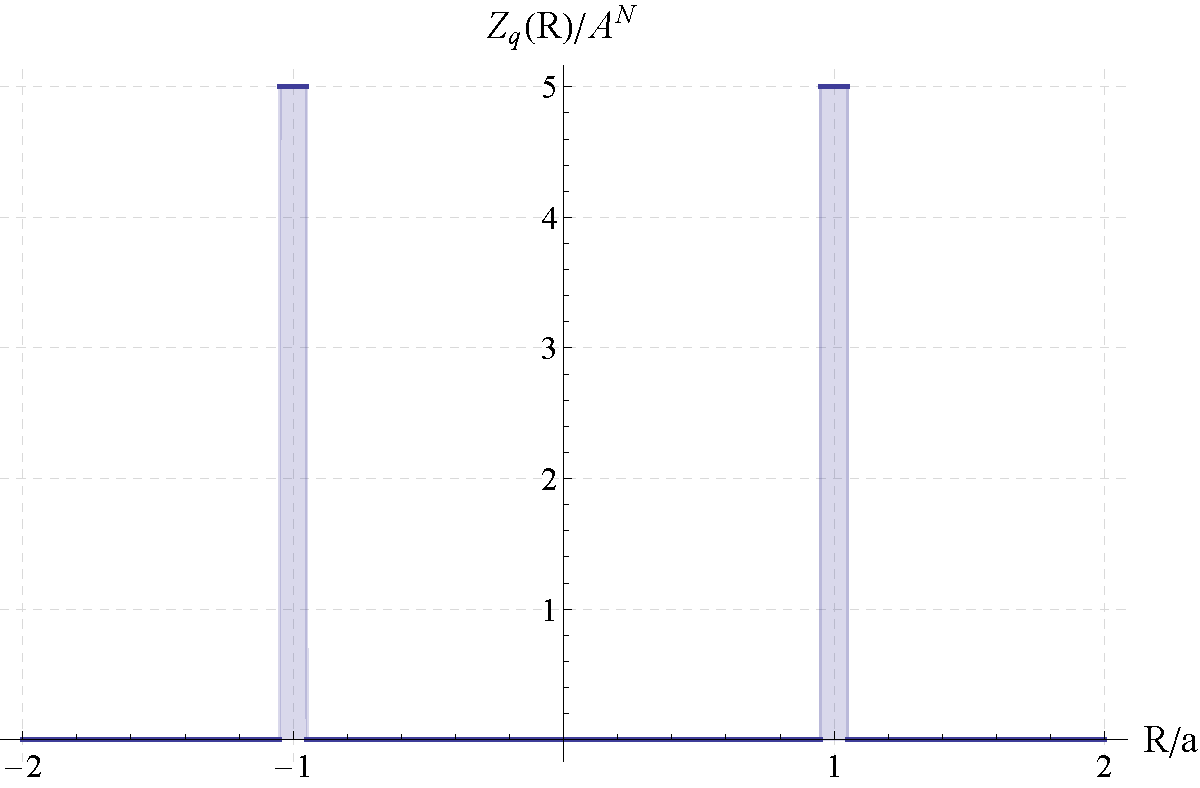
\includegraphics[scale=0.35]{Graphics/1D/Original/1D_N1_Orig.pdf}} &
\subfloat[N=2]{\label{fig:1DN2Orig}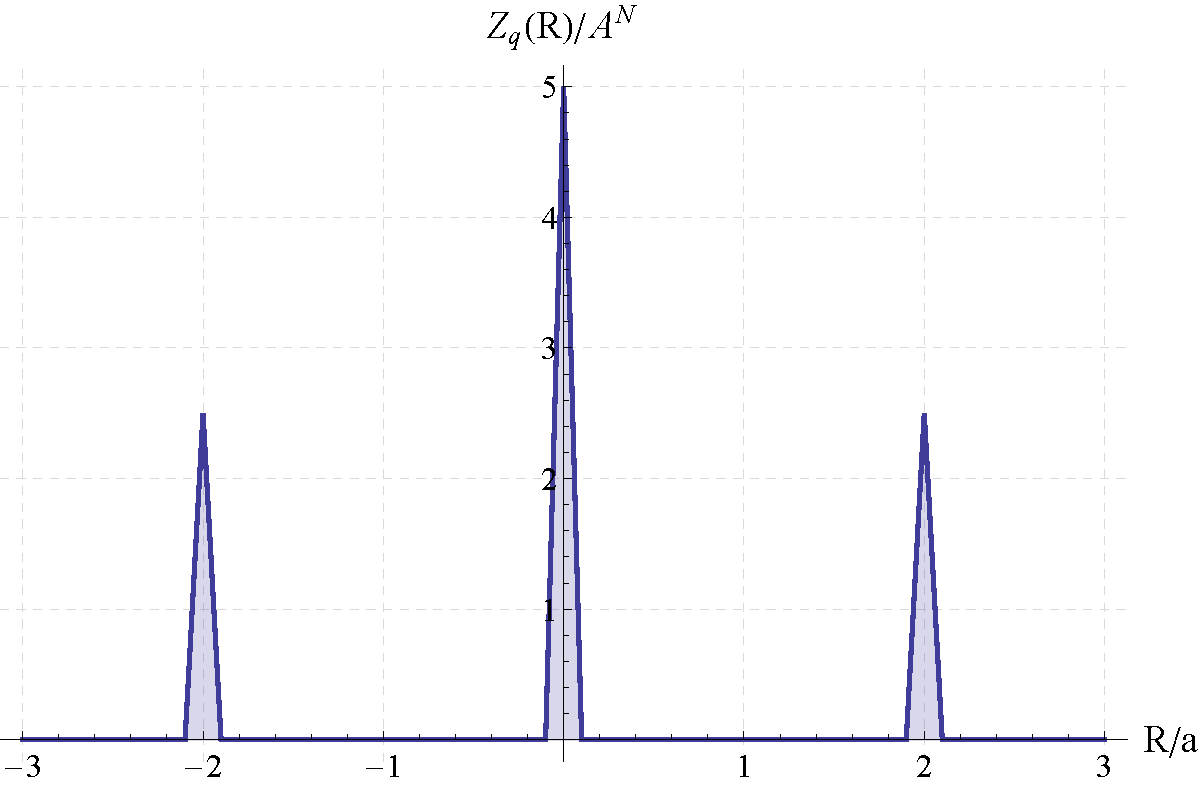
\includegraphics[scale=0.35]{Graphics/1D/Original/1D_N2_Orig.pdf}} \\
\subfloat[N=4]{\label{fig:1DN4Orig}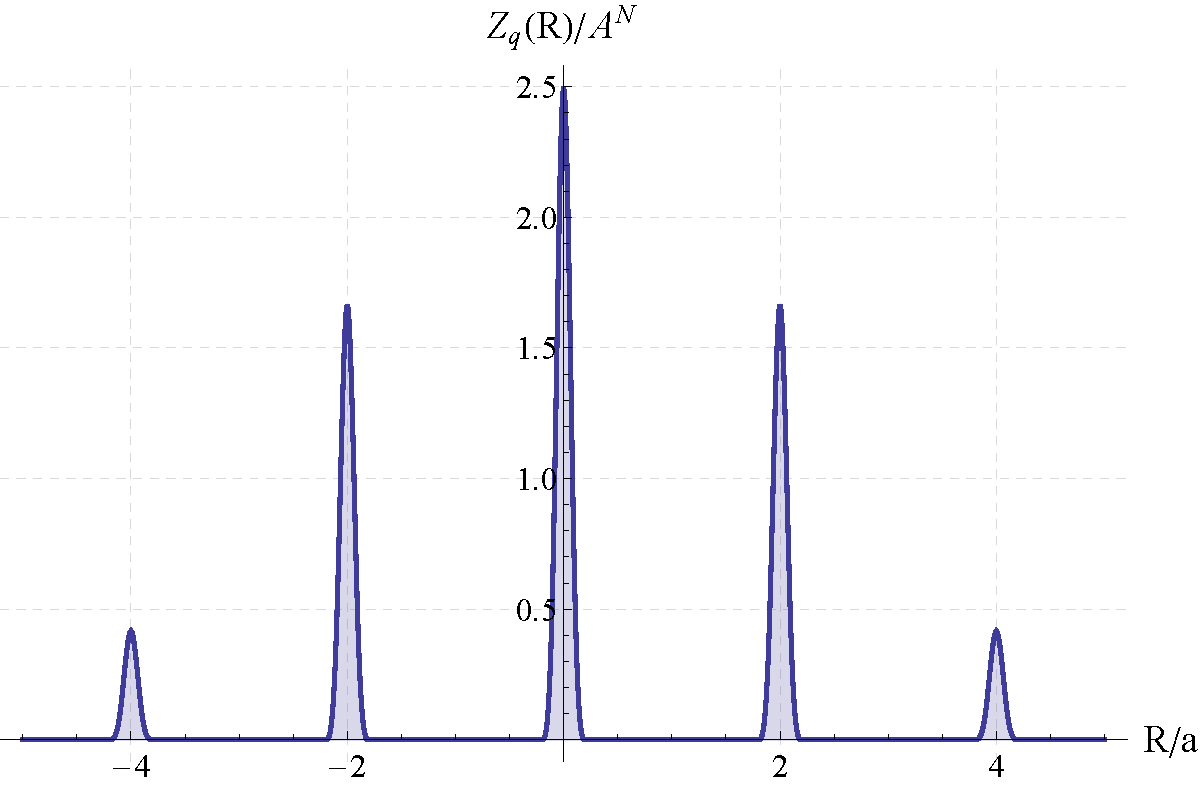
\includegraphics[scale=0.35]{Graphics/1D/Original/1D_N4_Orig.pdf}} &
\subfloat[N=6]{\label{fig:1DN6Orig}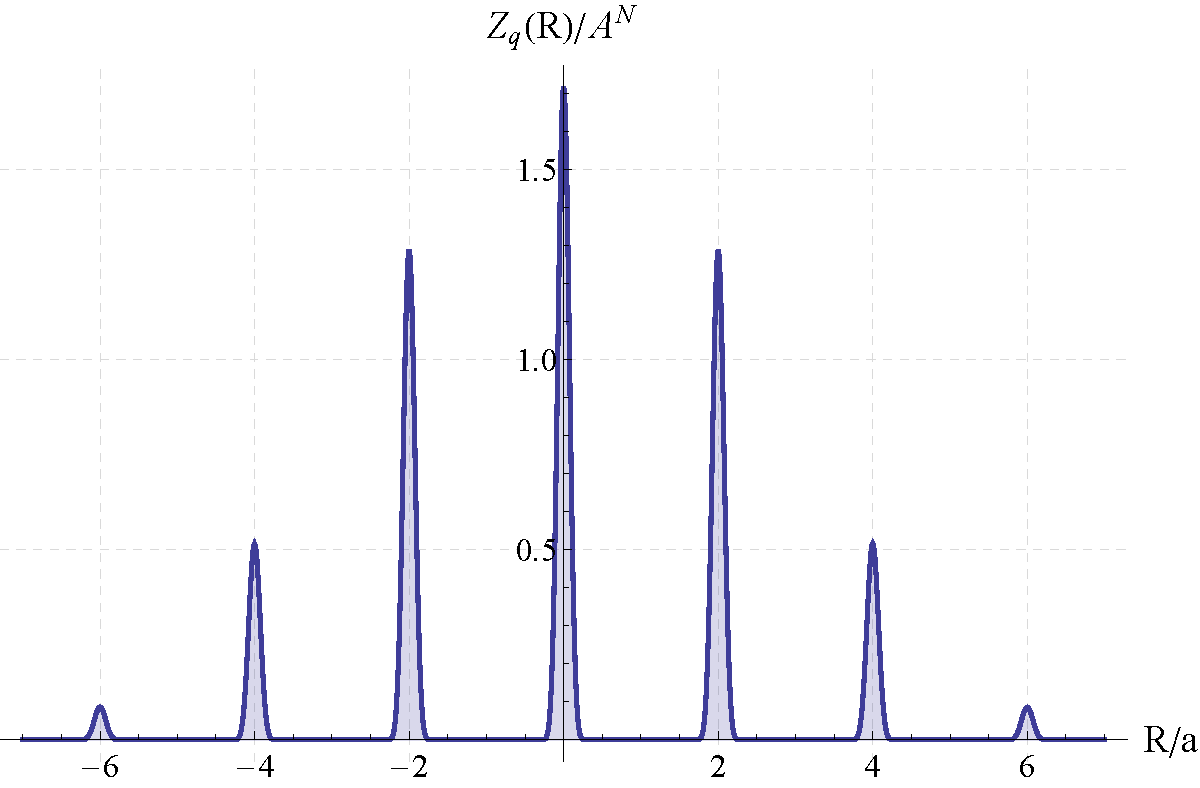
\includegraphics[scale=0.35]{Graphics/1D/Original/1D_N6_Orig.pdf}} \\
\subfloat[N=8]{\label{fig:1DN8Orig}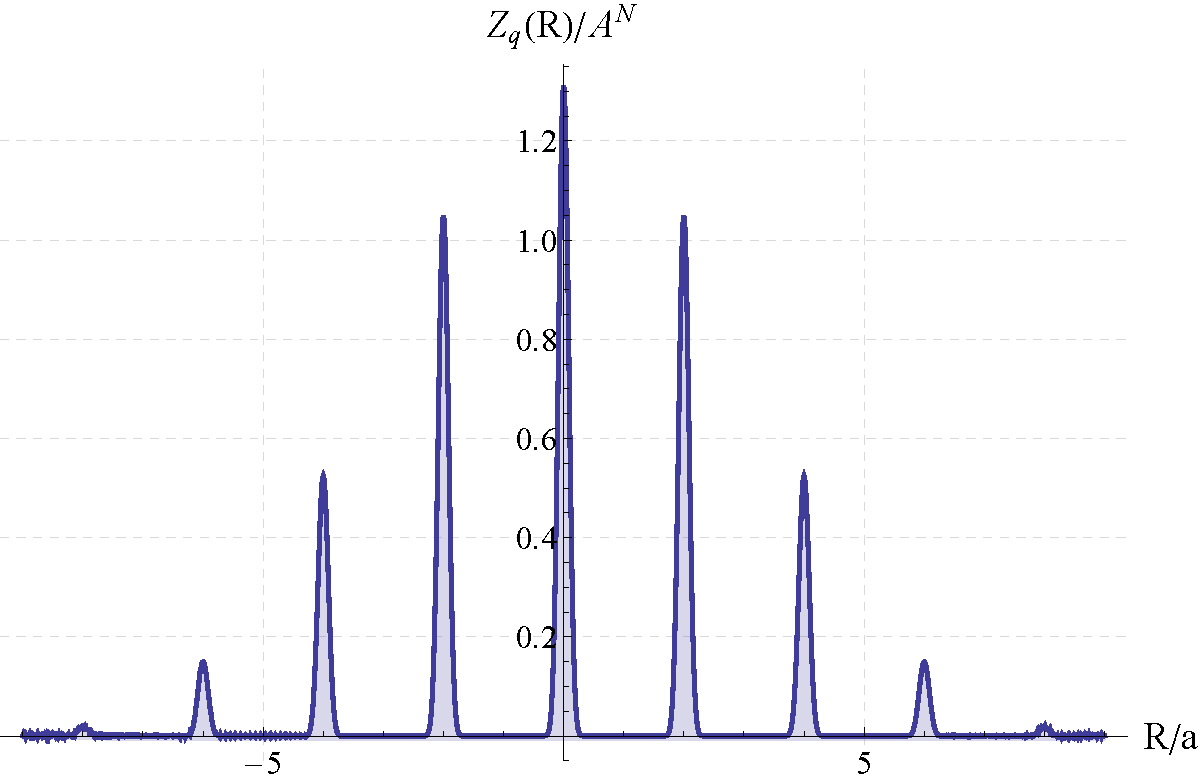
\includegraphics[scale=0.35]{Graphics/1D/Original/1D_N8_Orig.pdf}} &
\subfloat[N=10]{\label{fig:1DN10Orig}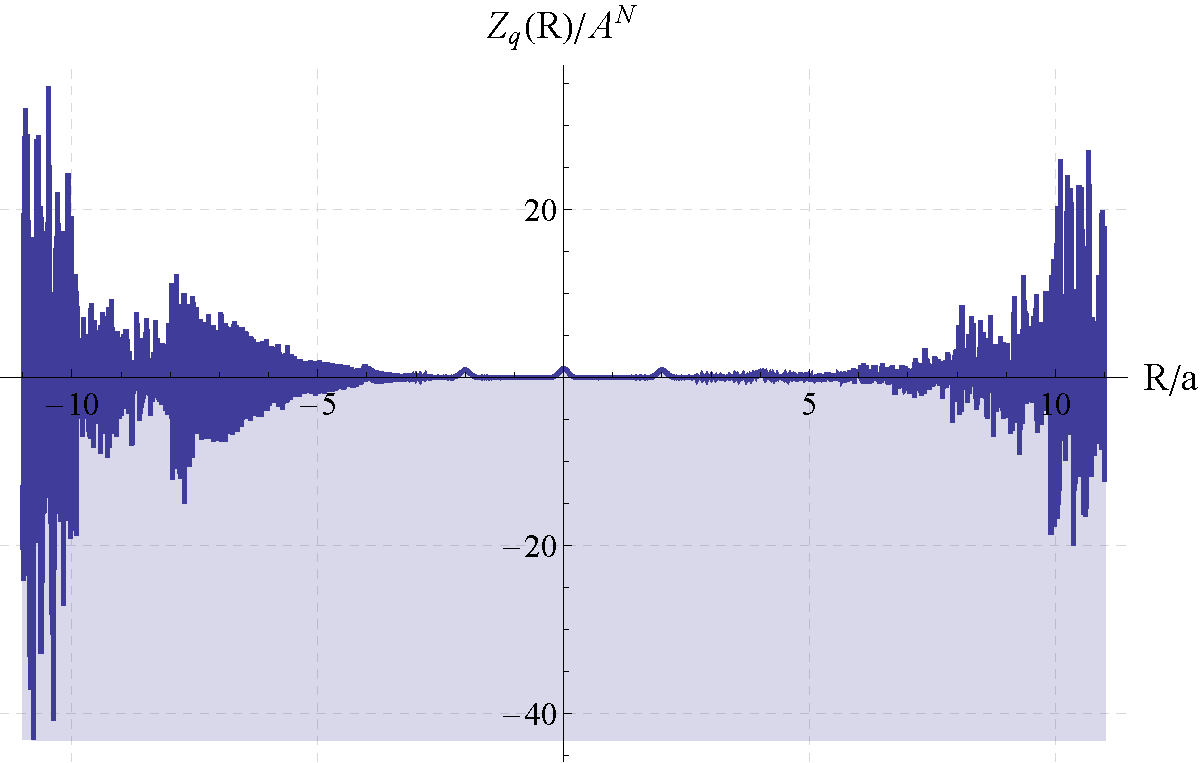
\includegraphics[scale=0.35]{Graphics/1D/Original/1D_N10_Orig.pdf}}
\end{tabular} 
\caption{Plots showing the partition function for an extendable FJC with $p=0.1a$. The original partition function used to plot these graphs \eqref{PartitionFunction1DSolved}. Notice the breakdown in the calculations for $N=10$.}
\label{fig:Z1DOrig} 
\end{figure}

\begin{figure}[htp]
\centering
\begin{tabular}{cc}
\subfloat[N=1]{\label{fig:1D_N1}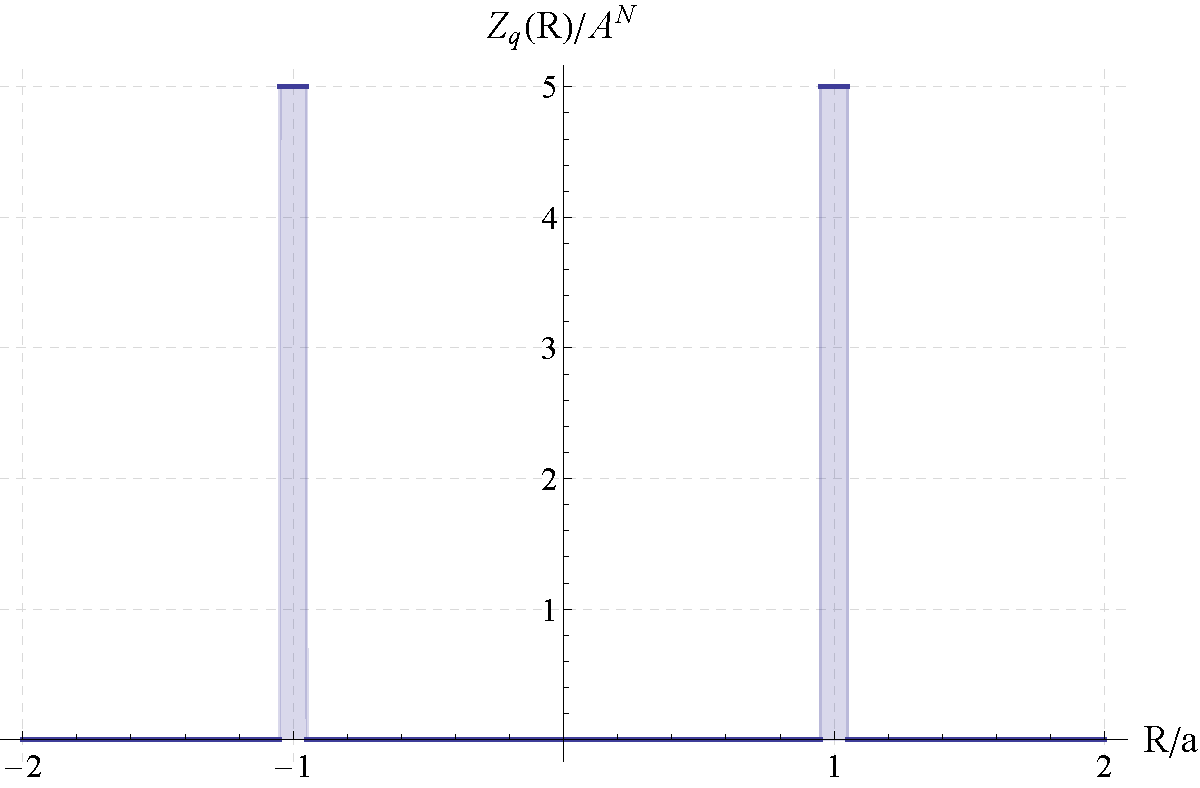
\includegraphics[scale=0.35]{Graphics/1D/1D_N1.pdf}} &
\subfloat[N=2]{\label{fig:1DN2}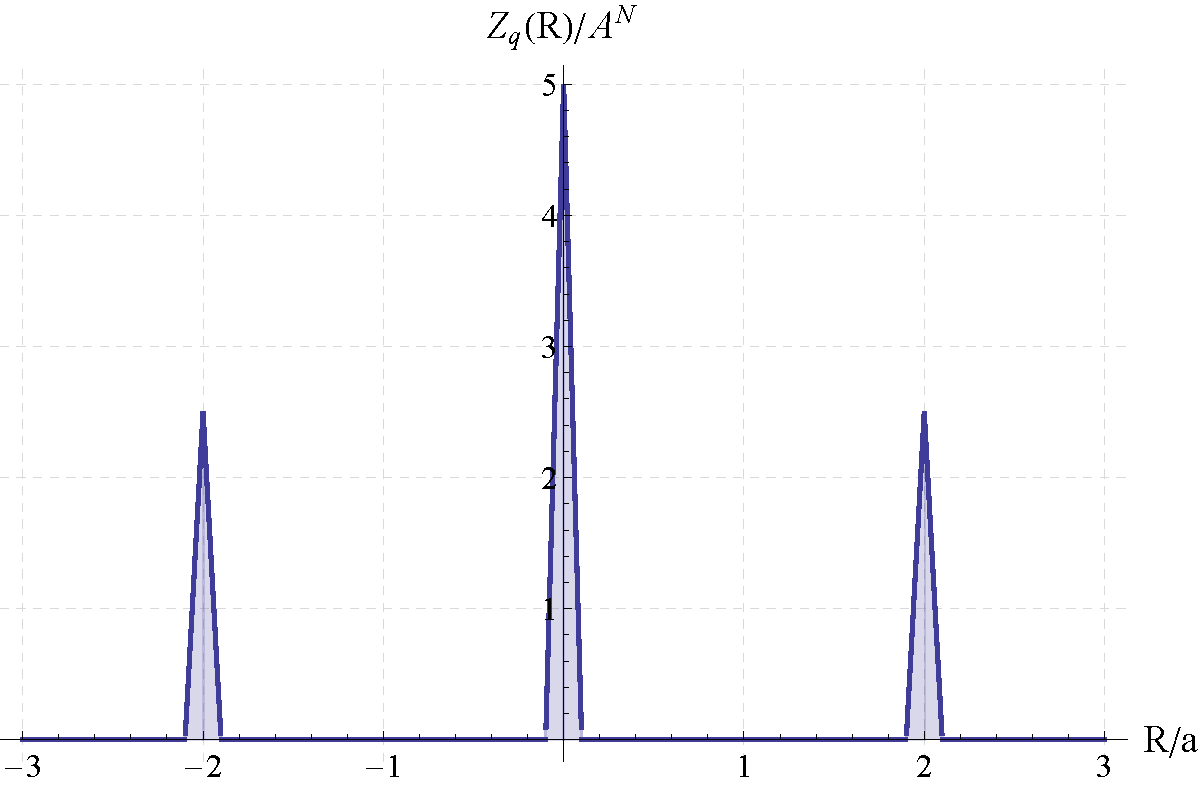
\includegraphics[scale=0.35]{Graphics/1D/1D_N2.pdf}} \\
\subfloat[N=4]{\label{fig:1DN4}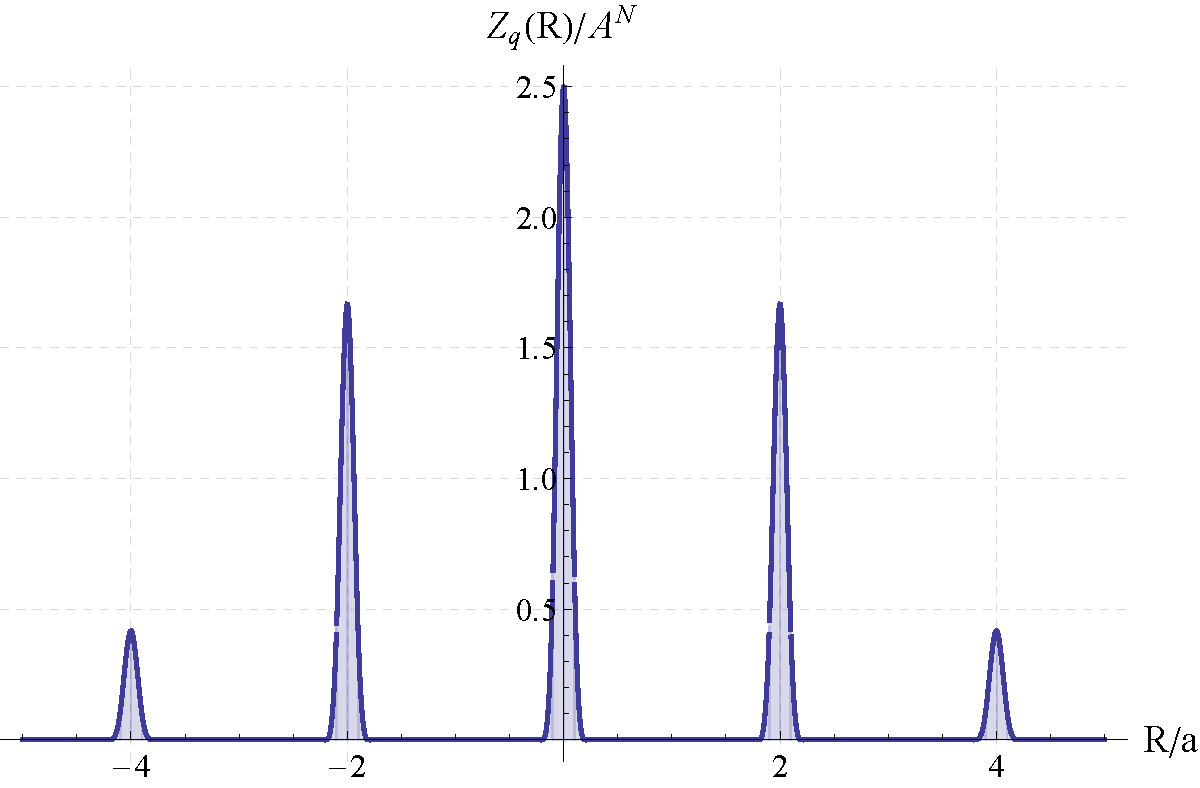
\includegraphics[scale=0.35]{Graphics/1D/1D_N4.pdf}} &
\subfloat[N=6]{\label{fig:1DN6}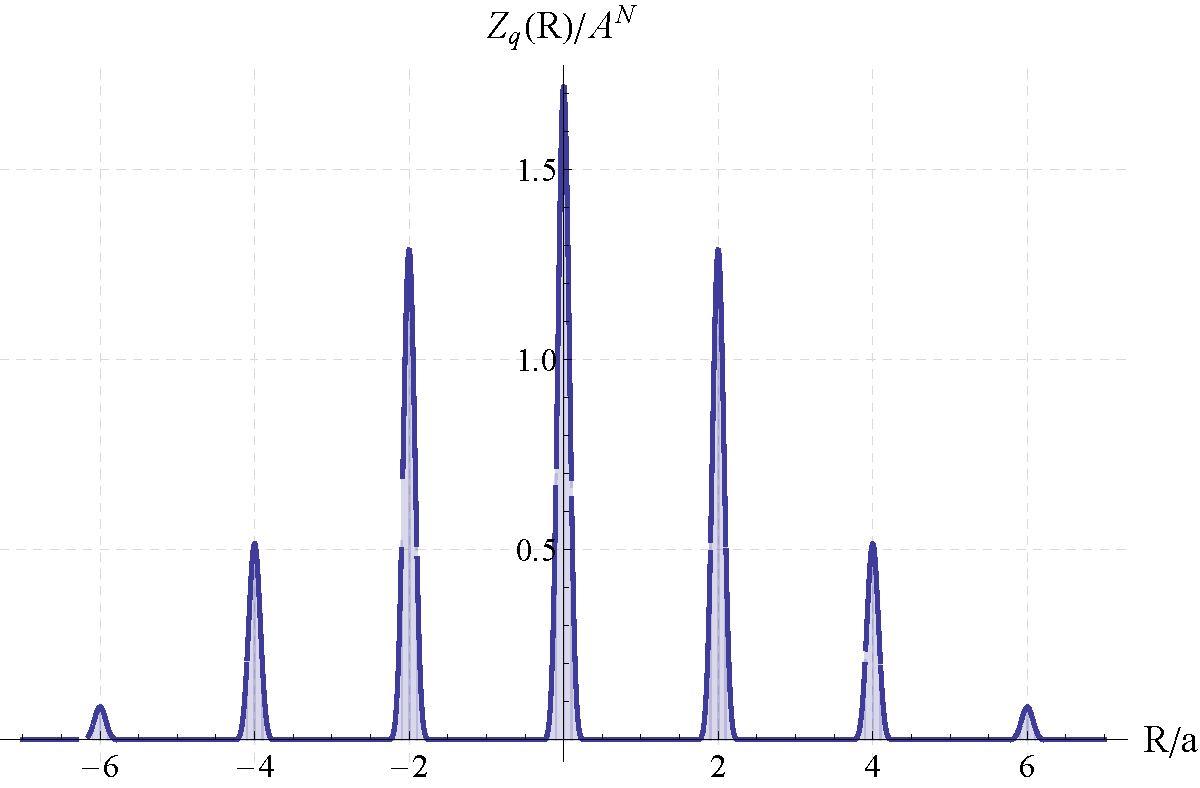
\includegraphics[scale=0.35]{Graphics/1D/1D_N6.pdf}} \\
\subfloat[N=8]{\label{fig:1DN8}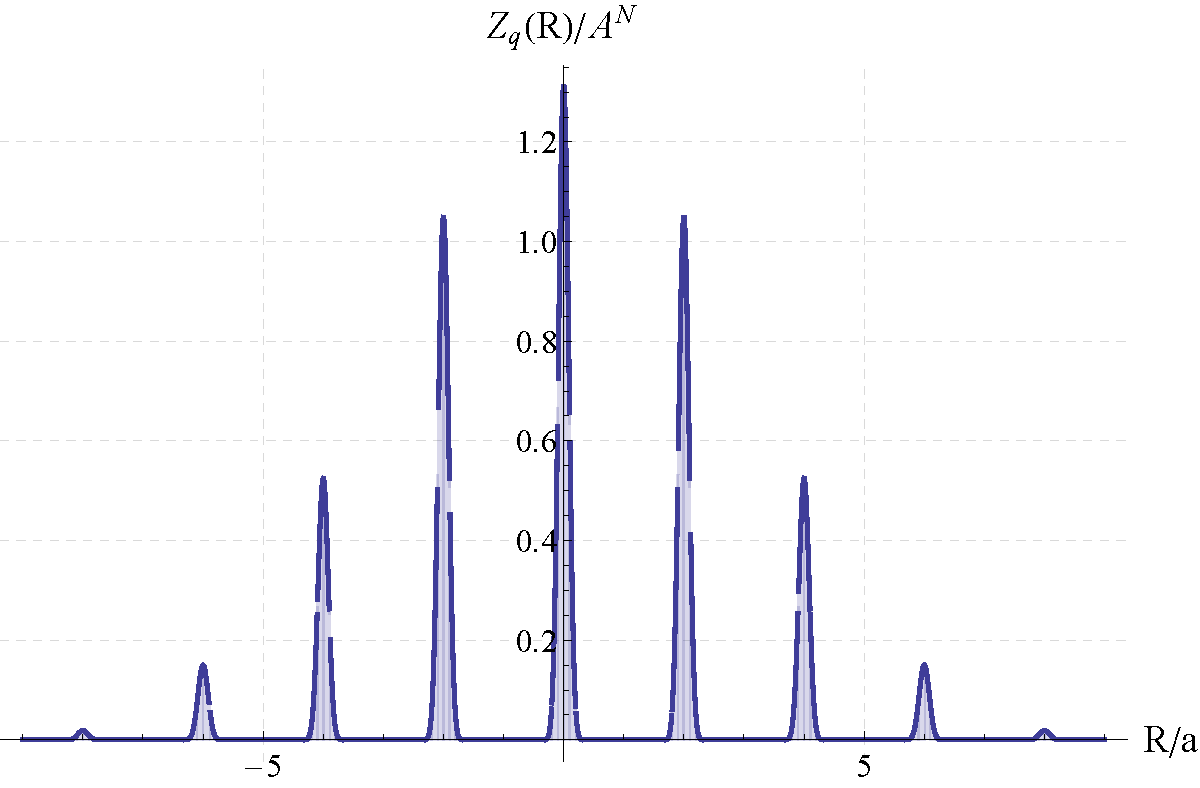
\includegraphics[scale=0.35]{Graphics/1D/1D_N8.pdf}} &
\subfloat[N=10]{\label{fig:1DN10}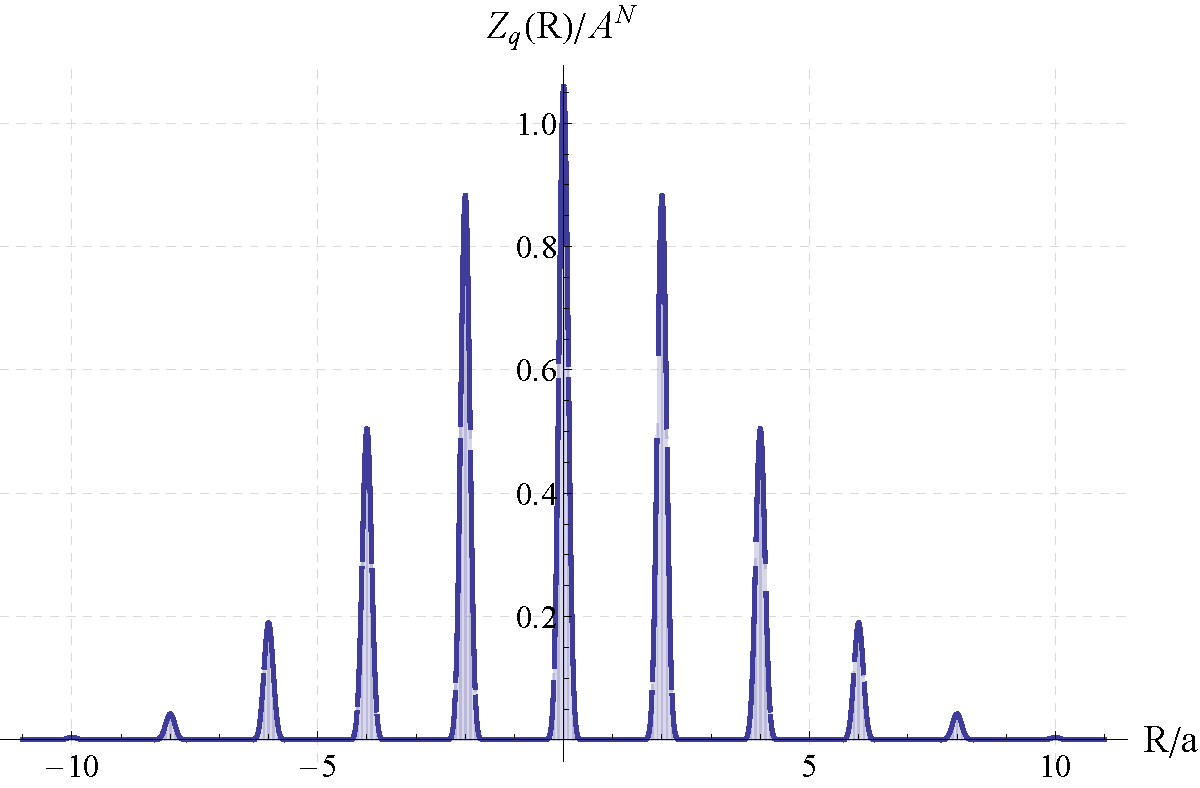
\includegraphics[scale=0.35]{Graphics/1D/1D_N10.pdf}}
\end{tabular} 
\caption{Plots showing the partition function for an extendable FJC with $p=0.1a$. The partition
function used to plot these graphs has been modified with the insertion of the top-hat function $\Theta(R,k)$. Notice that the failure to cancel terms in the expression has been avoided and the calculation for N=10 converges.}
\label{fig:Z1D} 
\end{figure}

\newpage
\section{Extendable Freely Jointed Chain in Three Dimensions}

Evaluating the partition function for a one dimensional EFJC gave an expression for $Z_{q}(R)$ which with slight adjustment worked well to give a probability density distribution for the end-to-end separation of the EFJC. In the small approximation of $p$, we saw that the behaviour of $Z_{q}$ tended towards that of a non-extendable FJC, consistent with the treatment of the FJC as a one dimensional random walk. Modelling the FJC as a stochastic process we were able to determine an expectation of $R$. The results were consistent with each other. The next stage is to take a 3-D realisation of the EFJC model, allowing each link to move independently in three spatial dimensions, employing a finite potential to characterise the links.

\subsection{Construction of the Partition Function}

In three dimensional space the current partition function integral is inadequate as it has been constructed in the Cartesian co-ordinate system. A better method would be to employ spherical co-ordinates where one end of the EFJC is fixed at the origin. We have
%
\begin{equation}
Z_{q}=\int \prod_{i=1}^{N}d^{3}\boldsymbol{r}_{i} \exp\left(-\frac{\Phi\left(\{\boldsymbol{r}_{i}\}\right)}{kT}\right)
\end{equation}
%
Each link in the 3D EFJC will be characterised by a potential which is function of $\boldsymbol{r}_{i,i-1}=\boldsymbol{r}_{i}-\boldsymbol{r}_{i-1}$, with $\boldsymbol{r}_{0}=0$, which allows it to extend or contract by a finite length $\frac{p}{2}$. This allows the potential, $\Phi$, to separate such that
%
\begin{equation}
\Phi\left(\{\boldsymbol{r}_{i}\}\right) = \sum_{i=1}^{N}\phi\left(\boldsymbol{r}_{i,i-1}\right)
\end{equation}
%
Inserting the constraint $\boldsymbol{r}'=\sum_{i=1}^{N}\boldsymbol{r}_{i,i-1}$ through a delta function, we fix the total vector sum of all the particle separations. We then define
%
\begin{equation}
Z_{q}\left(\boldsymbol{r}'\right)=\int\prod_{i=1}^{N}d^{3}\boldsymbol{r}_{i,i-1}\,\delta^{3}\left(\boldsymbol{r'}-\sum_{i=1}^{N}\boldsymbol{r}_{i,i-1}\right)\prod_{i=1}^{N} \exp\left(-\frac{\phi\left(\boldsymbol{r}_{i,i-1}\right)}{kT}\right)\label{pf3d1}
\end{equation}
%
such that $Z_{q}=\int Z_{q}\left(\boldsymbol{r}'\right)d^{3}\boldsymbol{r}'$.

Intuitively, we expect $Z_{q}\left(\boldsymbol{r}'\right)$ to depend on $R=|\boldsymbol{r}'|$ only. It counts the (weighted) numbers of configurations with polymer vector length $\boldsymbol{r}'$, and the orientation of $\boldsymbol{r}'$ does not alter this count. The probability distribution of the length $R$ is actually
%
\begin{equation}
P_{N}\left(R\right)= \frac{R^{2}Z_{q}\left(R\right)}{\int R^{2}Z_{q}\left(R\right)dR}
\end{equation}
%
which is correctly normalised such that $\int^{\infty}_{0} P_{N}\left(R\right)dR=1$. Using the integral representation of the delta function constraint as
%
\begin{equation}\label{pf3d_delta}
\delta\left(\boldsymbol{r}'-\sum_{i=1}^{N}\boldsymbol{r}_{i,i-1}\right)=\frac{1}{\left(2\pi\right)^{3}}\int d^{3}\boldsymbol{k}\, \exp\left(-i\boldsymbol{k}.\left(\boldsymbol{r}'-\sum_{i=1}^{N}\boldsymbol{r}_{i,i-1}\right)\right)
\end{equation}
%
and inserting it into \eqref{pf3d1} we obtain
%
\begin{equation}\label{pf3draw}
Z_{q}\left(\boldsymbol{r}'\right) = \frac{1}{\left(2\pi\right)^{3}}\int d^{3}\boldsymbol{k}\, \exp\left(-i\boldsymbol{k}.\boldsymbol{r}'\right)\left(\int_{-\infty}^{\infty}d^{3}\boldsymbol{r}_{i,i-1}\, \exp\left(-\frac{\phi\left(\boldsymbol{r}_{i,i-1}\right)}{kT}\right)\exp\left(i\boldsymbol{k}.\boldsymbol{r}_{i,i-1}\right) \right)^{N}
\end{equation}
%
Representing the Fourier transform of the weighting function as $F\left(\boldsymbol{k}\right)$, we can simplify \eqref{pf3draw} so that it becomes a function of $R$,
%
\begin{align}
Z_{q}\left(R\right) &= \frac{1}{\left(2\pi\right)^{3}}\int_{0}^{\infty}k^{2}\left(2\pi\int_{-1}^{1} e^{-ikR\cos \theta} d\left(\cos \theta \right)\right)dk\, F^{N}\left(\boldsymbol{k}\right) \\
&= \frac{1}{\left(2\pi\right)^{2}}\int_{0}^{\infty}dk\frac{k}{R}\sin kR\, F^{N}\left(\boldsymbol{k}\right)\label{PartitionFunctionUnsolved3D} 
\end{align}
%
where the Fourier transform integral $F\left(\boldsymbol{k}\right)$ is
%
\begin{equation}
F\left(\boldsymbol{k}\right)=\int_{-\infty}^{\infty}d^{3}\boldsymbol{r}_{i,i-1}\, \exp\left(-\frac{\phi\left(\boldsymbol{r}_{i,i-1}\right)}{kT}\right)\exp\left(i\boldsymbol{k}.\boldsymbol{r}_{i,i-1}\right)\label{FTPI_3D}
\end{equation}
%
Using this general expression for $Z_{q}\left(R\right)$ any potential may be studied.  

\subsection{Evaluating $\boldsymbol{Z_{q}}$ for the non-extendable Freely Jointed Chain}

We previously calculated the partition function for a FJC in one dimension using two delta functions as the weighting factor. Performing the calculation in three dimensions
the analogous potential as a function of $r = |\boldsymbol{r}_{i,i-1}|$ is
%
\begin{equation}
\phi\left(\boldsymbol{r}_{i,i-1}\right)=-kT\ln\left(D\delta\left(r-a\right)\right)\label{FJC3D}
\end{equation}
%
Where $D$ is a constant with dimensions of length. Inserting \eqref{FJC3D} into \eqref{FTPI_3D} we get
%
\begin{align}
F\left(\boldsymbol{k}\right) & =\int_{-\infty}^{\infty}\int_{-\infty}^{\infty}\int_{-\infty}^{\infty}\, d^{3}\boldsymbol{r}\,D\delta\left(r-a\right)\exp\left(-i\boldsymbol{k.r}\right)\nonumber\\
 & =D\int_{-1}^{1}2\pi d\left(\cos\theta\right)\int_{0}^{\infty}\delta\left(r-a\right)r^{2}\exp\left(-ikr\cos\theta\right)dr\nonumber\\
 & =D\int_{0}^{\infty}\delta\left(r-a\right)\frac{4\pi r}{k}\sin kr\,dr\label{FJC_FTP_Unsolved}
\end{align}
%
Such that the Fourier transform of the exponentiated potential for a FJC becomes
%
\begin{equation}
F\left(k\right)=\left(\frac{4\pi a D}{k}\right)\sin ka\label{FourierTransformPotentialWeighted}
\end{equation}
%
Inserting \eqref{FourierTransformPotentialWeighted} into \eqref{PartitionFunctionUnsolved3D}
the partition function integral becomes
%
\begin{equation}
Z_{q}\left(R\right) = \frac{\left(4 \pi a D\right)^{N}}{4\pi^{2}R} \int_{0}^{\infty}\frac{\sin kR \sin^{N}ka}{k^{N-1}}\,dk
\end{equation}
%
and using \eqref{Sin_Series} to express $\sin^{N}ka$ as a sum of exponentials and $\sin kR$ as the real part of $ie^{-ikR}$ the partition function becomes
%
\begin{equation}
Z_{q}\left(R\right) = \frac{\left(4 \pi a D\right)^{N}i}{4\pi^{2}R \left(2i\right)^{N}}\sum^{N}_{l=0}\binom{N}{l}\left(-1\right)^{l}\int^{\infty}_{0}\frac{e^{ik\left(a\left(N-2l\right)-R\right)}}{k^{N-1}}\,dk
\end{equation}
%
Since the integral has already been calculated in \eqref{MultipoleIntegral}, the solution for a FJC in 3-D becomes
%
\begin{equation}
Z_{q}\left(R\right)=\frac{\left(2\pi a D\right)^{N}}{4\pi R\left(N-2\right)!}\sum_{l=0}^{N}\binom{N}{l}\left(-1\right)^{l}\left[a\left(N-2l\right)-R\right]^{N-2}\sgn\left(a\left(N-2l\right)-R\right)\label{PartitionFunction3DFJC}
\end{equation}

\subsection{The Shell Potential and its Fourier Transform}

In the 1-D model we saw that a double top-hat weighting function was able to generate the partition function for an EFJC. In three dimensions, due to the rotational symmetry the potential is only dependent on the $r$ co-ordinate. A potential that is non-zero only within the range of $r$ at $a-\frac{p}{2}\leq r\leq a+\frac{p}{2}$ gives a weighting function that can be viewed as a shell with a thickness of length $p$.

Working with the partition function, let us insert $\exp\left(-\phi\left(r\right)/kT\right)=C$ for $a-\frac{p}{2}\leq r\leq a+\frac{p}{2}$, and zero elsewhere, $\exp\left(-\phi\left(r\right)/kT\right)=0$, where $C$ is a dimensionless constant. Contributions to the partition function arise only where the potential is finite so the exponentiated potential Fourier transform integral simplifies to
%
\begin{equation}
F\left(k\right)=C\int_{\cos\theta=-1}^{1}2\pi d\left(\cos\theta\right)\int_{a-\frac{p}{2}}^{a+\frac{p}{2}}r^{2}dr\, e^{ikr\cos\theta}
\end{equation}
%
This result was obtained by using $d^{3}\boldsymbol{r}=d\phi\sin\theta d\theta r^{2}dr$ and rewriting $\sin\theta d\theta$ as $-d\left(\cos\theta\right)$. Performing the integral with respect to $r$ in the potential range
we have the final result
%
\begin{equation}
F\left(k\right)=\frac{4\pi C}{k^{2}}\left(\frac{2\cos ka\sin\frac{kp}{2}}{k}+2a\sin ka\sin\frac{kp}{2}-p\cos ka\cos\frac{kp}{2}\right)\label{PotentialTerm3D}
\end{equation}
%
With this expression for $F\left(k\right)$ the final partition function for a EFJC can be analytical evaluated in 3-D.

\subsection{Evaluation of the Partition Function by the small $p$ approximation}

In the small $p$ approximation we once again insert Taylor expansions of all the trigonometric functions in the Fourier transform potential with respect to $p$. For small $p$ in \eqref{PotentialTerm3D} we have a much simpler equation for $F\left(k\right)$
%
\begin{equation}
F\left(k\right)=C\left(\frac{4\pi a p}{k}\right)\sin ka\label{PotentialTerm3DApprox}
\end{equation}
%
Using \eqref{PotentialTerm3DApprox} with \eqref{PartitionFunctionUnsolved3D}
we get
%
\begin{equation}
Z_{q}\left(R\right)=\frac{\left(4\pi a p C\right)^{N}}{2\pi^{2}R}\int_{-\infty}^{\infty}\frac{\sin kR}{k^{N-1}}\sin^{N}ka\, dk
\end{equation}
%
Which evaluates to give
%
\begin{equation}
Z_{q}\left(R\right)=\frac{\left(2\pi a p C\right)^{N}}{2\pi R\left(N-2\right)!}\sum_{l=0}^{N}\binom{N}{l}\left(-1\right)^{l}\left[a\left(N-2l\right)-R\right]^{N-2}\sgn\left(a\left(N-2l\right)-R\right)\label{PartitionFunction3DSmallp}
\end{equation}
%
From the plot in \figref{PF3D} we see that in the large $N$ limit the partition function with constrained end-to-end separation $R$ gives a distribution that peaks about the origin. This is expected for the behaviour of
a FJC. \figref{PF3Dn} shows the probability density function of the end-to-end separation. 
%
\begin{figure}[htp]
 \centering 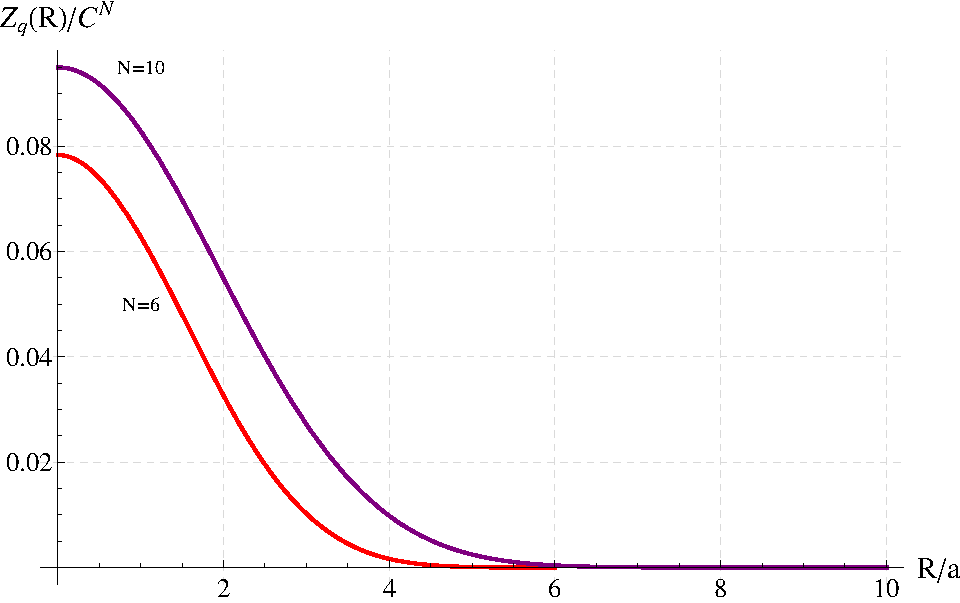
\includegraphics[scale=0.6]{Graphics/PartitionFunction3D.pdf} 
\caption{A plot of \eqref{PartitionFunction3DFJC} for $N=6,10$.}
\label{fig:PF3D} 
\end{figure}

\begin{figure}[htp]
\centering 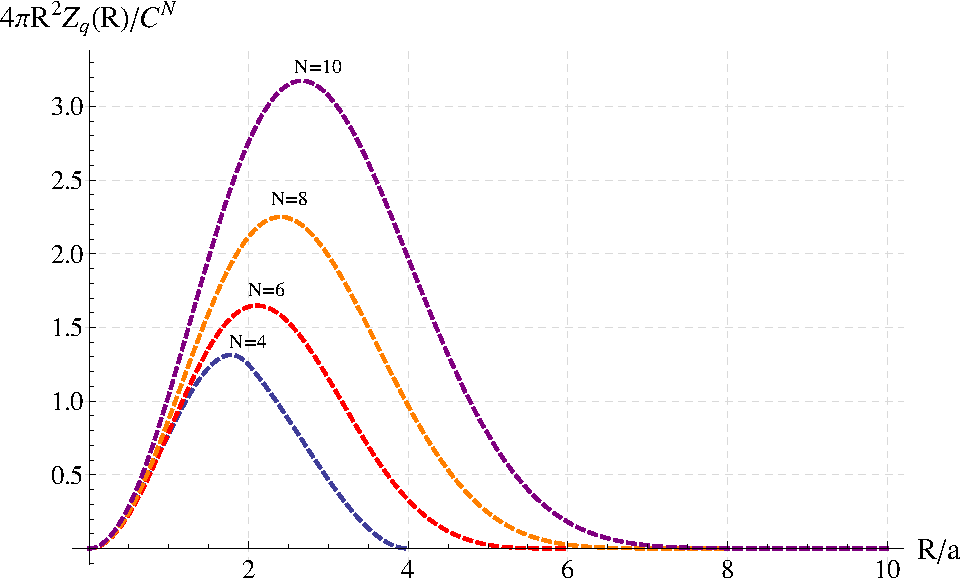
\includegraphics[scale=0.6]{Graphics/PartitionFunction3Dn.pdf} 
\caption{A plot of \eqref{PartitionFunction3DFJC} multiplied by $4\pi R^{2}$
for $N=4,6,8,10$.}
\label{fig:PF3Dn} 
\end{figure}

\subsection{Evaluating the Partition Function for arbitrary $p$}

In the previous section we saw that when the small $p$ approximation was applied to the EFJC in one dimension the resulting partition function became a description of the FJC, a similar case was seen when the small approximation was made in three dimensions. Let us now evaluate the partition function for the EFJC without approximation. We have the Fourier transform as an exact expression, and to combine the various terms into a single complex integral we can first use the binomial theorem to collect the terms which have different factors of $\frac{1}{k}$
%
\begin{equation}
F^{N}(k)=\left(2\pi C\right)^{N}\sum_{\alpha=0}^{N}\binom{N}{\alpha}\frac{1}{i^{\alpha}}\frac{1}{k^{2N+\alpha}}X^{\alpha}Y^{N-\alpha}
\end{equation}
%
where
%
\begin{equation}
X=e^{ik\left(a+\frac{p}{2}\right)}-e^{ik\left(a-\frac{p}{2}\right)}+e^{ik\left(-a+\frac{p}{2}\right)}-e^{ik\left(-a-\frac{p}{2}\right)}
\end{equation}
%
and
%
\begin{equation}
Y=\left(-a-\frac{p}{2}\right)e^{ik\left(a+\frac{p}{2}\right)}-\left(-a+\frac{p}{2}\right)e^{ik\left(a-\frac{p}{2}\right)}+\left(a-\frac{p}{2}\right)e^{ik\left(-a+\frac{p}{2}\right)}-\left(a+\frac{p}{2}\right)e^{ik\left(-a-\frac{p}{2}\right)}
\end{equation}
%
The multinomial theorem is then used for the $X^{\alpha}$ and $Y^{N-\alpha}$ terms. This approach reduces the terms to a single exponent as a function of $k$ such that the integral over $dk$ is simplified. Combining this result with \eqref{PartitionFunctionUnsolved3D} we get a final expression for $Z_{q}$ as
%
\begin{equation}
Z_{q}(R)=\frac{\pi \left(-1\right)^{N}\left(2\pi\right)^{N-2}C^{N}}{R}\sum_{\alpha=0}^{N}\binom{N}{\alpha}\frac{1}{\left(2N+\alpha-2\right)!}\sum_{j_{1},j_{2},j_{3},j_{4}}^{\alpha}\sum_{l_{1},l_{2},l_{3},l_{4}}^{N-\alpha}I\left(N,\alpha,a,p,R,\{j\},\{l\}\right)
\label{PartitionFunctionFiniteP}
\end{equation}
%
with
%
\begin{multline}
I\left(N,\alpha,a,p,R,\{j\},\{l\}\right)=\binom{N}{j_{1},j_{2},j_{3},j_{4}}\binom{N-\alpha}{l_{1},l_{2},l_{3},l_{4}}\left(-1\right)^{j_{2}+j_{4}}\left(-a-\frac{p}{2}\right)^{l_{1}+l_{4}} \times \\ \left(a-\frac{p}{2}\right)^{l_{2}+l_{3}}\left(J\left(a,p,\{j\}\right)+L\left(a,p,\{l\}\right)-R\right)^{2N+\alpha-2}\sgn\left(J\left(a,p,\{j\}\right)+L\left(a,p,\{l\}\right)-R\right)
\end{multline}
%
and
%
\begin{eqnarray*}
\binom{N}{j_{1},j_{2},j_{3},j_{4}}&=&\frac{N!}{j_{1}!\,j_{2}!\,j_{3}!\,j_{4}!} \\
\binom{N-\alpha}{l_{1},l_{2},l_{3},l_{4}}&=&\frac{\left(N-\alpha\right)!}{l_{1}!\,l_{2}!\,l_{3}!\,l_{4}!}
\end{eqnarray*}
%
\begin{eqnarray*}
L\left(a,p,\{l\}\right)&=&\left(a+\frac{p}{2}\right)\left(l_{1}-l_{4}\right)+\left(a-\frac{p}{2}\right)\left(l_{2}-l_{3}\right) \\
J\left(a,p,\{j\}\right)&=&\left(a+\frac{p}{2}\right)\left(j_{1}-j_{4}\right)+\left(a-\frac{p}{2}\right)\left(j_{2}-j_{3}\right)
\end{eqnarray*}
%
\begin{eqnarray*}
\sum^{4}_{k=1}j_{k}&=&N \\
\sum_{k=1}^{4}l_{k}&=&N-\alpha
\end{eqnarray*}
%
A plot of \eqref{PartitionFunctionFiniteP} in \figref{Z3DMultigraphNormailsed} shows
the probability distributions for $N=3,4,5,6$. As $N$ increases in \figref{Z3D} we see that the distributions increasingly centre around $r=0$. \figref{3D_N5} show results for large $N$, where we begin to see that the results become unstable just like in \figref{1DN8Orig}.

\begin{figure}[H]
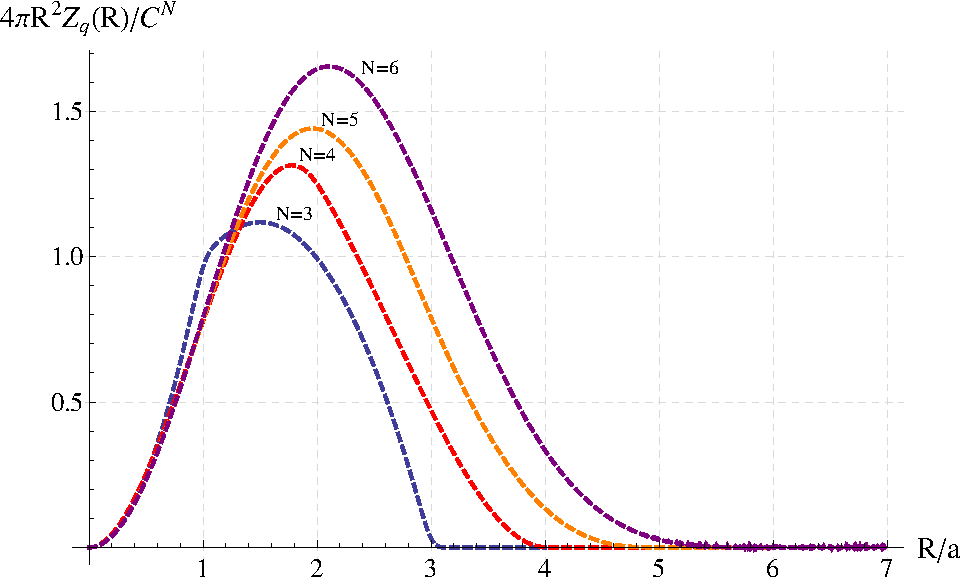
\includegraphics[scale=0.8]{Graphics/3D/MultigraphFinitePSmall.pdf}
\caption{A plot of normalised partition functions for an extendable FJC in three dimensions. The plot shows distributions for $N=3,4,5,6$ with $p=0.1a$.}
\label{fig:Z3DMultigraphNormailsed}
\end{figure}

\begin{figure}[H]
\centering
\begin{tabular}{cc}
\subfloat[N=1]{\label{fig:3D_N1}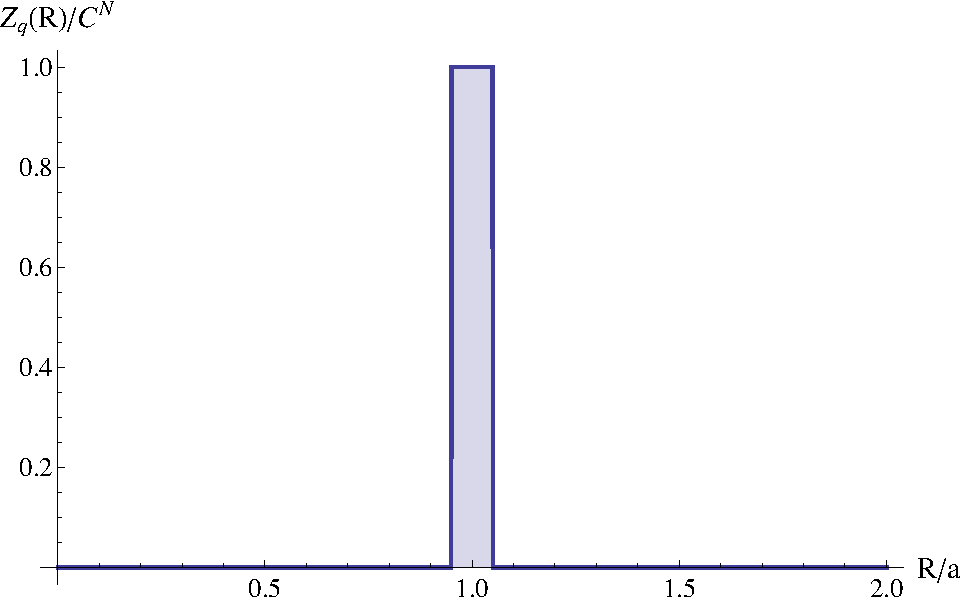
\includegraphics[scale=0.45]{Graphics/3D/FinitePSmall/1.pdf}} &
\subfloat[N=2]{\label{fig:3D_N2}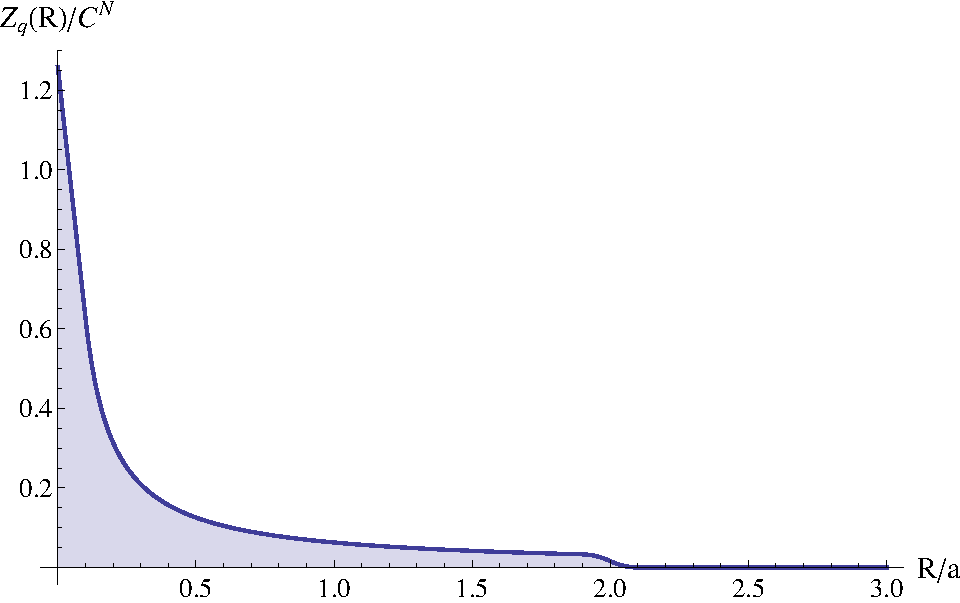
\includegraphics[scale=0.45]{Graphics/3D/FinitePSmall/2.pdf}} \\
\subfloat[N=3]{\label{fig:3D_N3}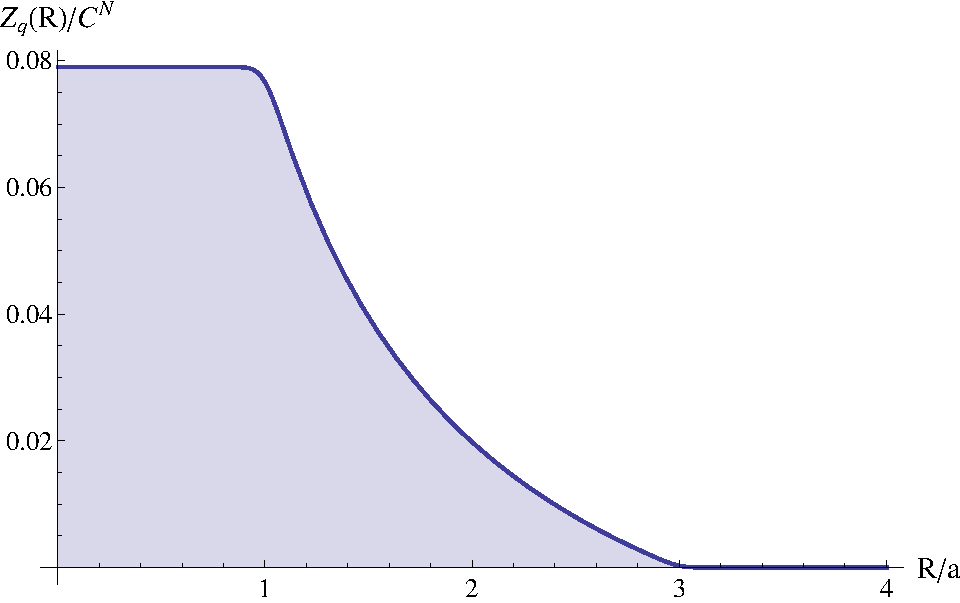
\includegraphics[scale=0.45]{Graphics/3D/FinitePSmall/3.pdf}} &
\subfloat[N=4]{\label{fig:3D_N4}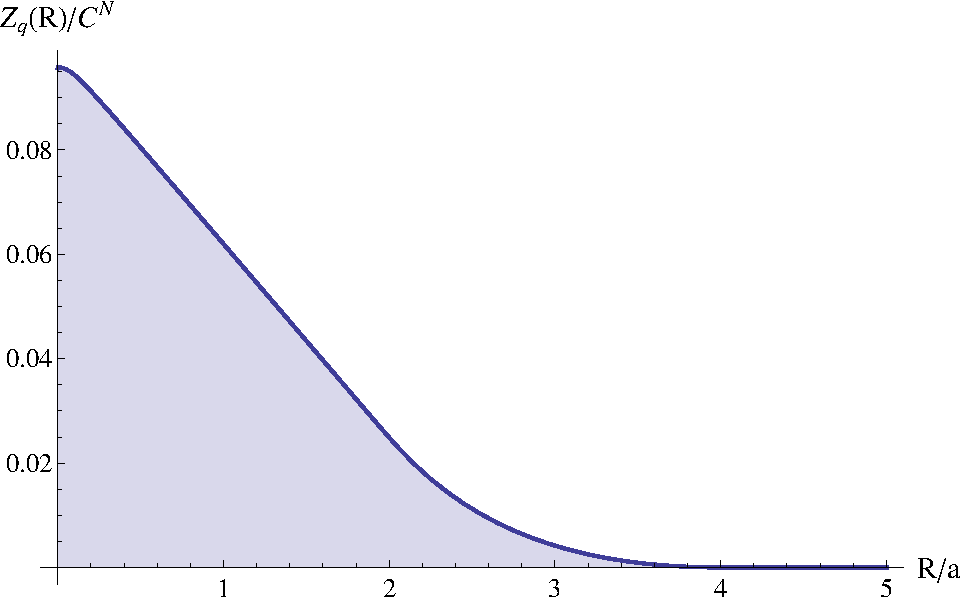
\includegraphics[scale=0.45]{Graphics/3D/FinitePSmall/4.pdf}} \\
\subfloat[N=5]{\label{fig:3D_N5}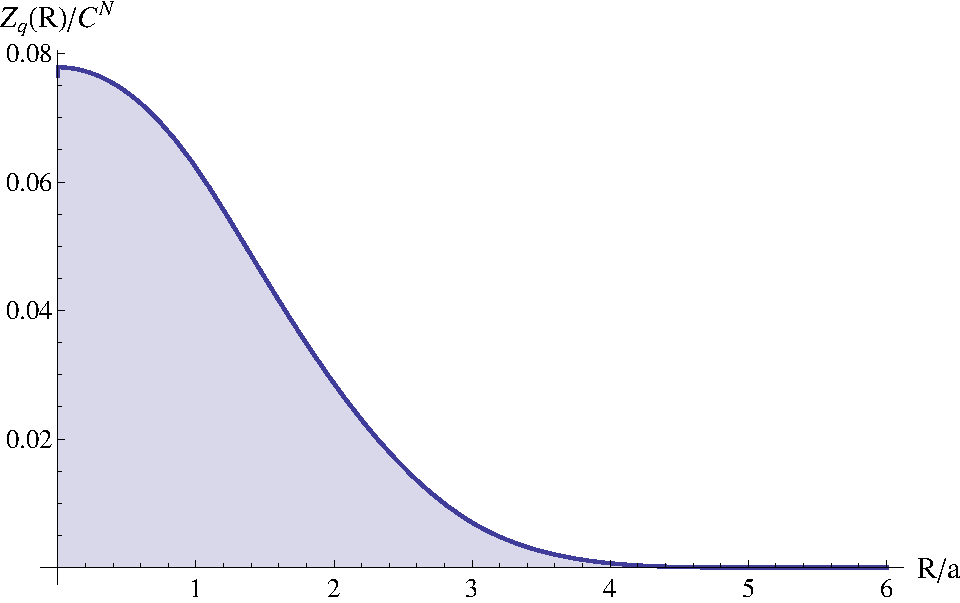
\includegraphics[scale=0.45]{Graphics/3D/FinitePSmall/5.pdf}} &
\subfloat[N=6]{\label{fig:3D_N6}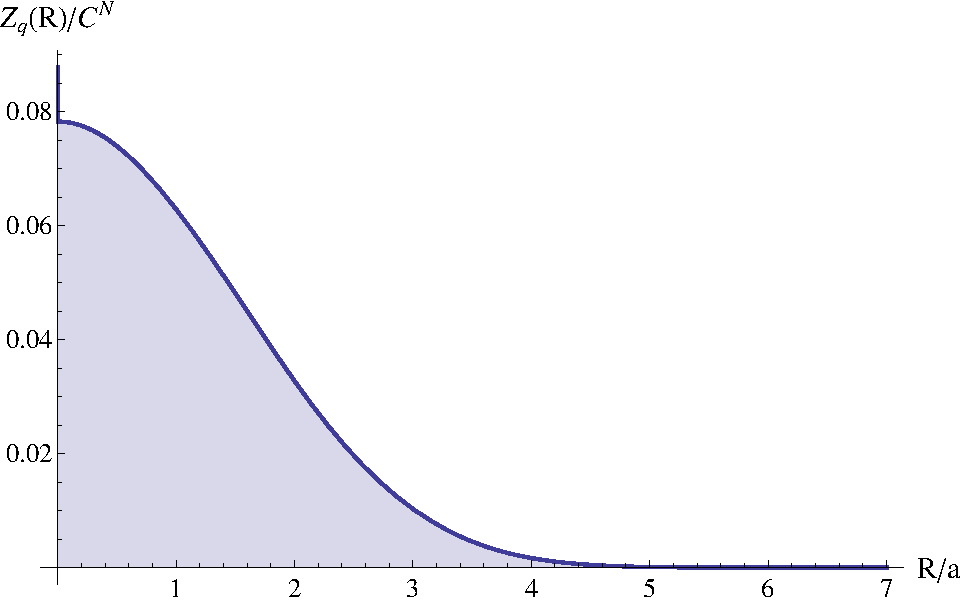
\includegraphics[scale=0.45]{Graphics/3D/FinitePSmall/6.pdf}} 
\end{tabular} 
\caption{Plots showing the partition function for an extendable FJC in three dimensions with $p=0.1a$.}
\label{fig:Z3D}
\end{figure}

\begin{comment}
\begin{figure}[H]
\centering
\begin{tabular}{cc}
\subfloat[N=1]{\label{fig:3D_N1Large}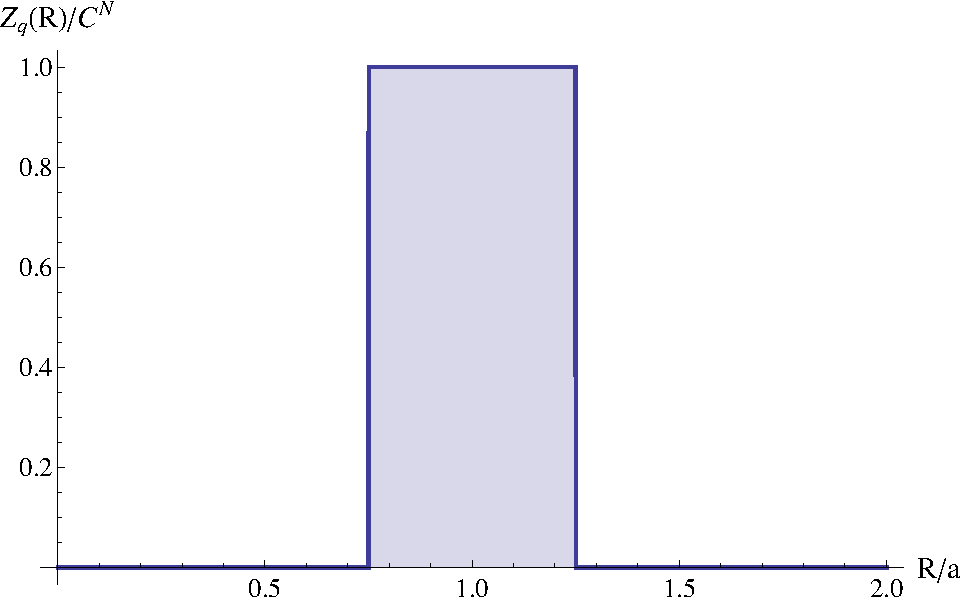
\includegraphics[scale=0.45]{Graphics/3D/FinitePLarge/1.pdf}} &
\subfloat[N=2]{\label{fig:3D_N2Large}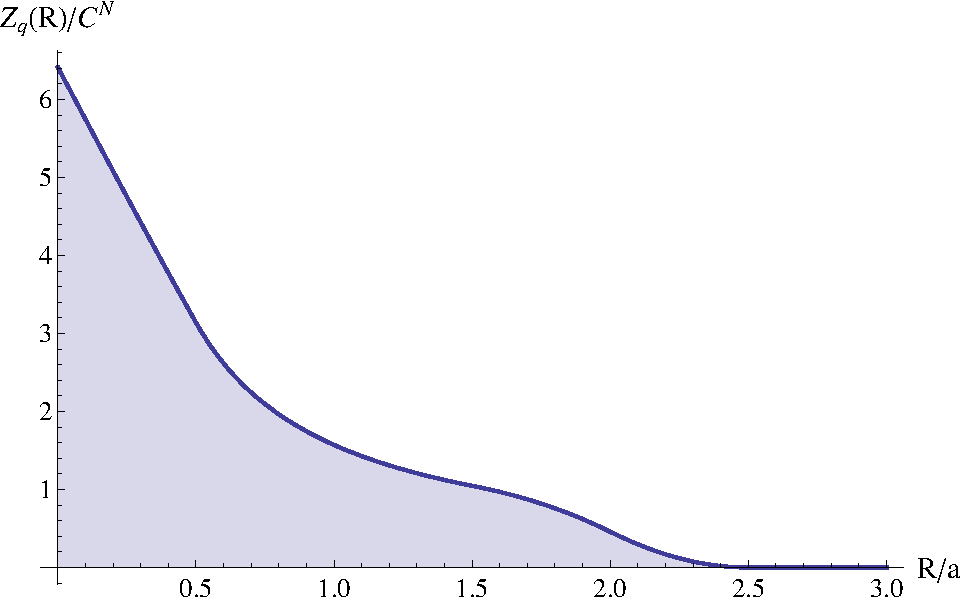
\includegraphics[scale=0.45]{Graphics/3D/FinitePLarge/2.pdf}} \\
\subfloat[N=3]{\label{fig:3D_N3Large}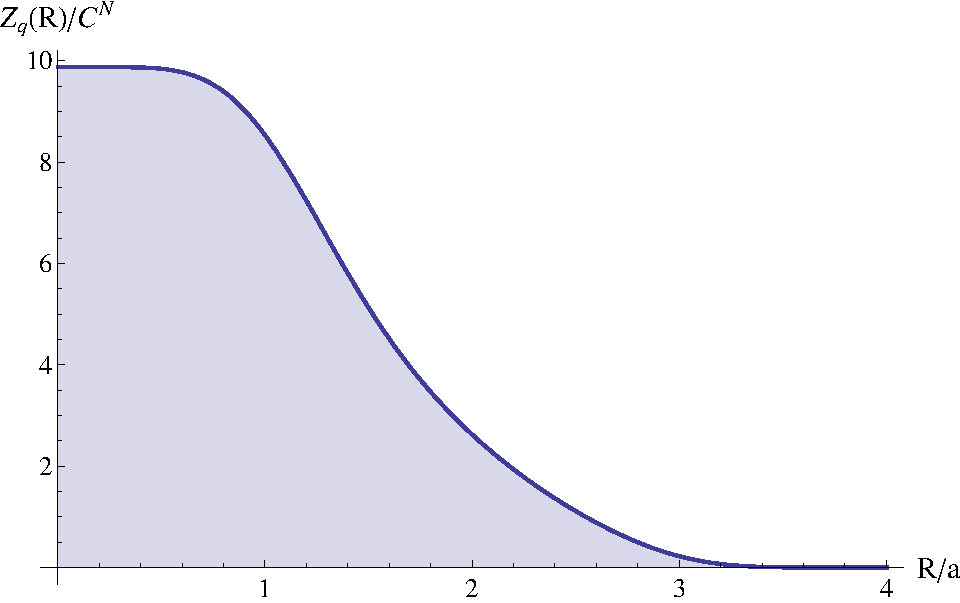
\includegraphics[scale=0.45]{Graphics/3D/FinitePLarge/3.pdf}} &
\subfloat[N=4]{\label{fig:3D_N4Large}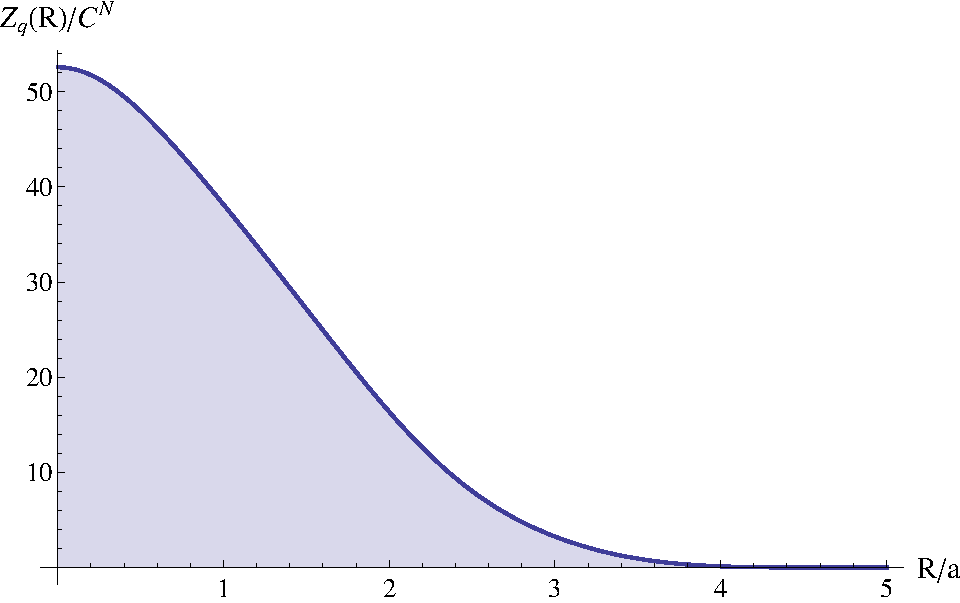
\includegraphics[scale=0.45]{Graphics/3D/FinitePLarge/4.pdf}} \\
\subfloat[N=5]{\label{fig:3D_N5Large}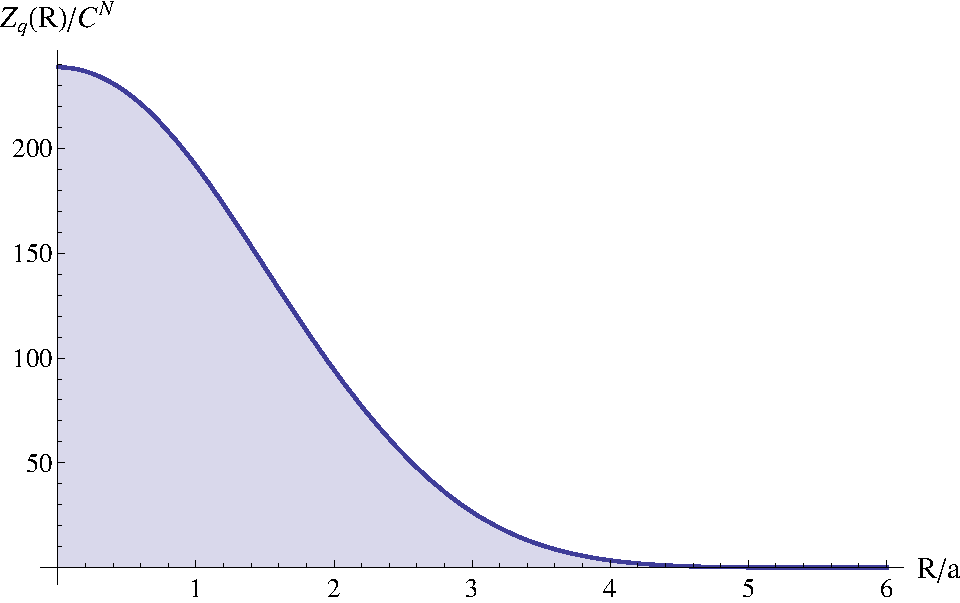
\includegraphics[scale=0.45]{Graphics/3D/FinitePLarge/5.pdf}} &
\subfloat[N=6]{\label{fig:3D_N6Large}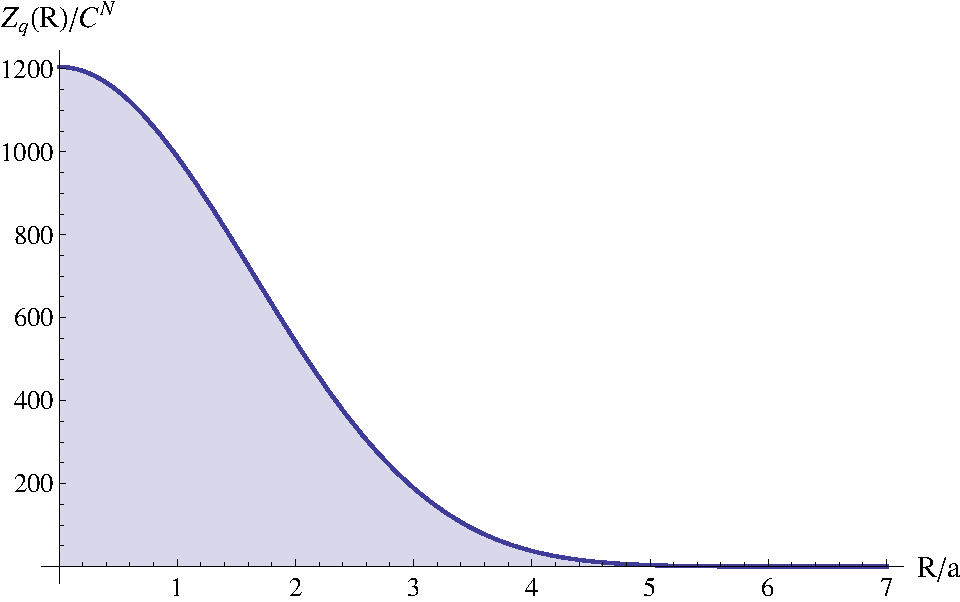
\includegraphics[scale=0.45]{Graphics/3D/FinitePLarge/6.pdf}} 
\end{tabular} 
\caption{Plots showing the partition function for an extendable FJC in three dimensions with $p=0.5a$.}
\label{fig:Z3DLarge}
\end{figure}
\end{comment}

\begin{figure}[H]
\centering
\begin{tabular}{cc}
\subfloat[p=0.1a]{\label{fig:3D_com01}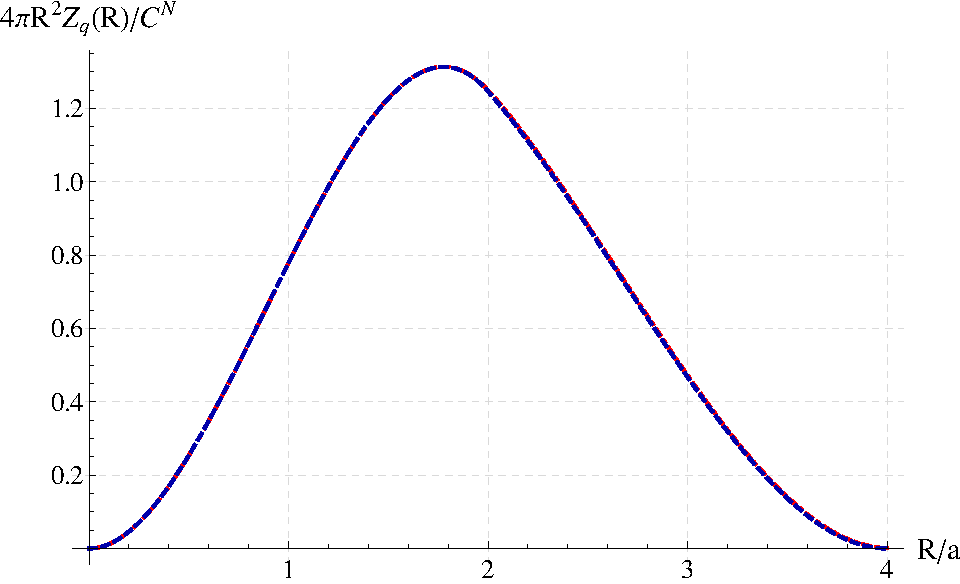
\includegraphics[scale=0.45]{Graphics/3D/Comparison/4_p01.pdf}} &
\subfloat[p=0.2a]{\label{fig:3D_com02}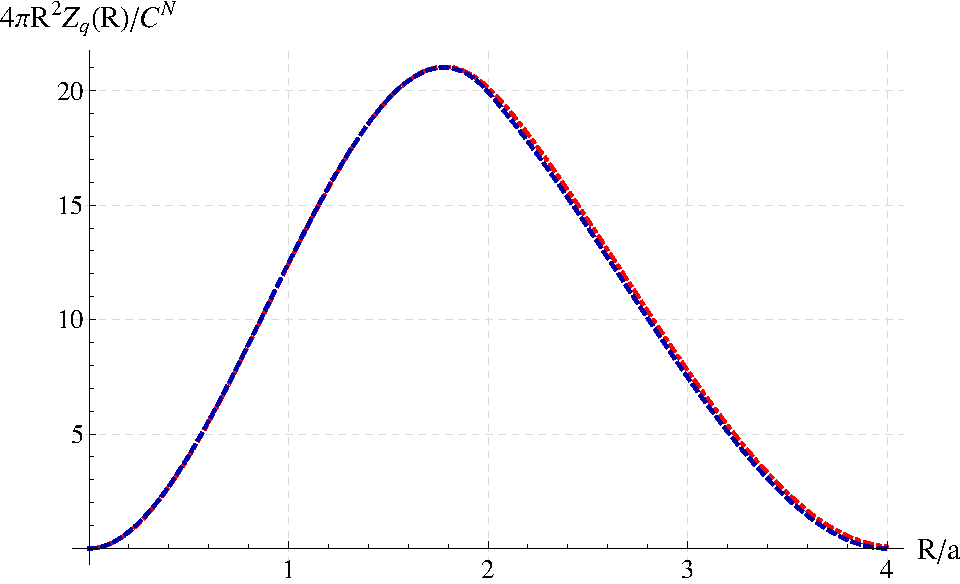
\includegraphics[scale=0.45]{Graphics/3D/Comparison/4_p02.pdf}} \\
\subfloat[p=0.3a]{\label{fig:3D_com03}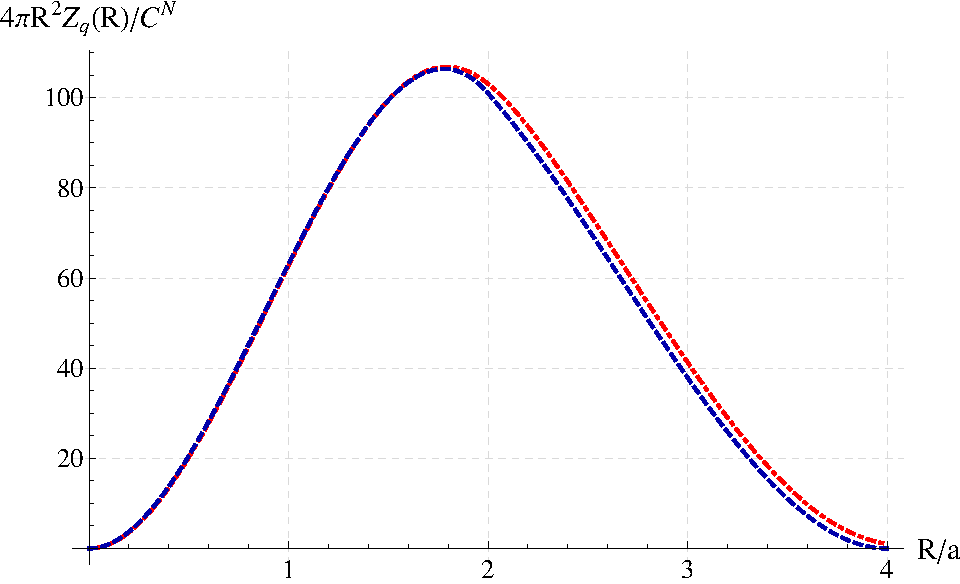
\includegraphics[scale=0.45]{Graphics/3D/Comparison/4_p03.pdf}} &
\subfloat[p=0.4a]{\label{fig:3D_com04}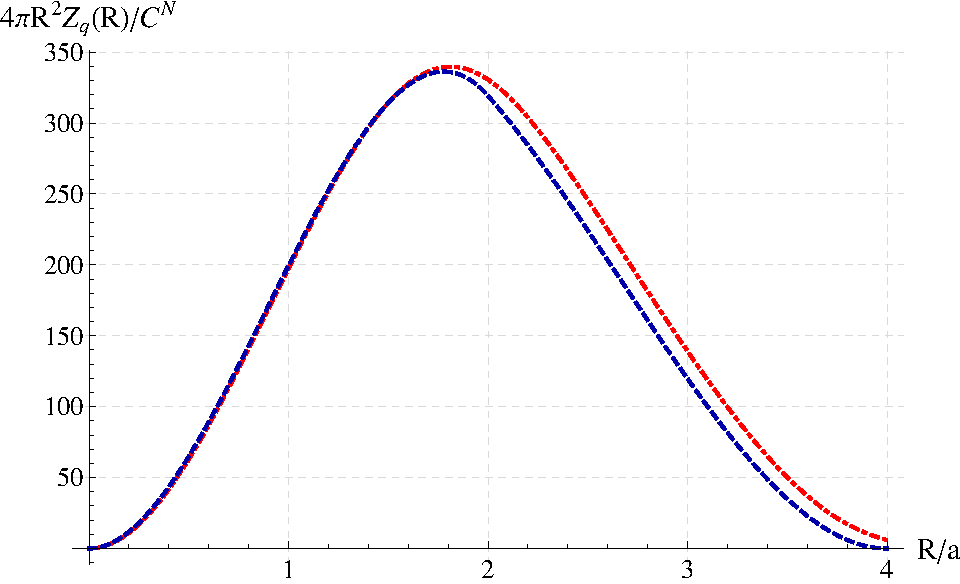
\includegraphics[scale=0.45]{Graphics/3D/Comparison/4_p04.pdf}} \\
\subfloat[p=0.5a]{\label{fig:3D_com05}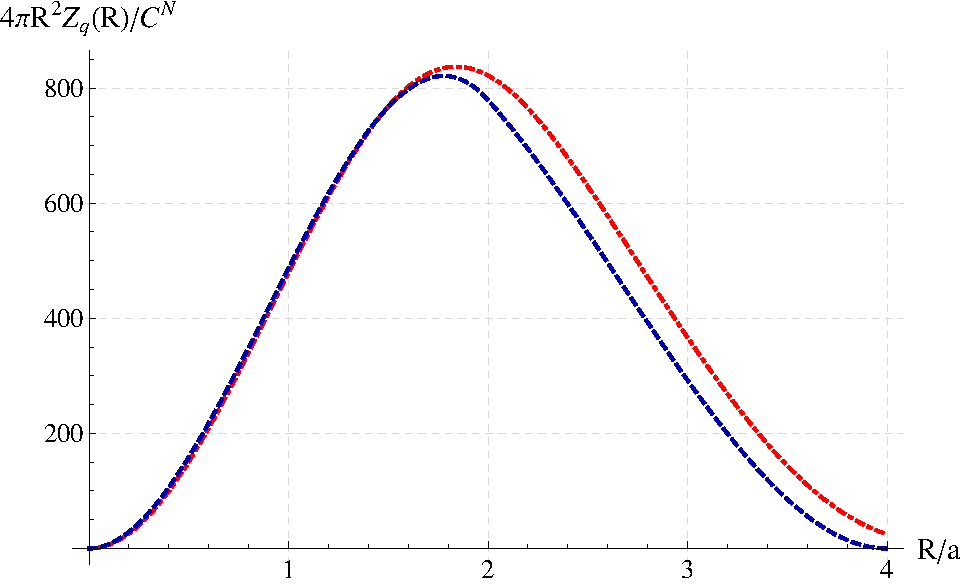
\includegraphics[scale=0.45]{Graphics/3D/Comparison/4_p05.pdf}} &
\subfloat[p=0.6a]{\label{fig:3D_com06}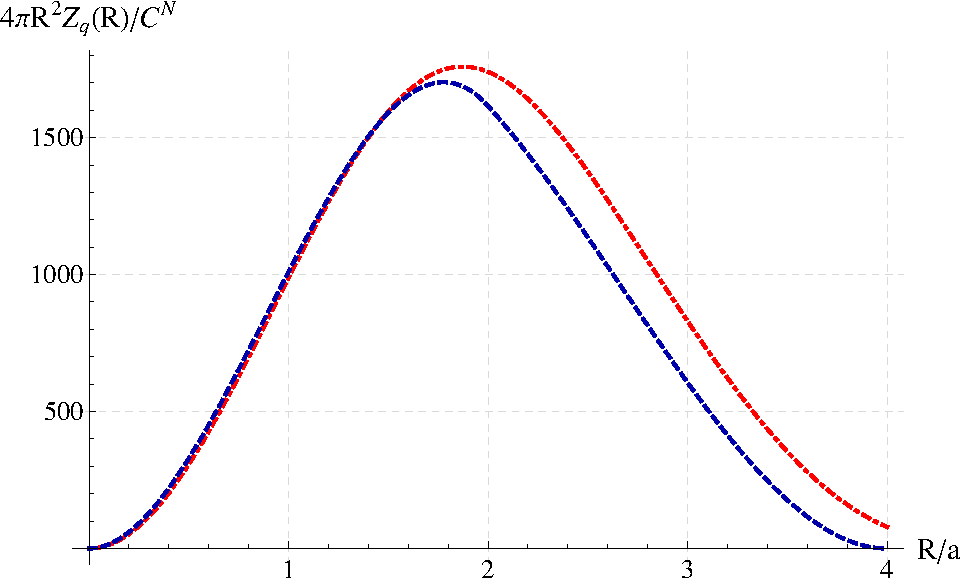
\includegraphics[scale=0.45]{Graphics/3D/Comparison/4_p06.pdf}}
\end{tabular} 
\caption{These plots show a comparison of the probability distribution for the FJC \eqref{PartitionFunction3DSmallp} (blue curve) and the EFJC \eqref{PartitionFunctionFiniteP} (red curve) for different values of $p$ with $N=4$.}
\label{fig:Comparison3D}
\end{figure}
\newpage
\begin{comment}
\begin{figure}[H]
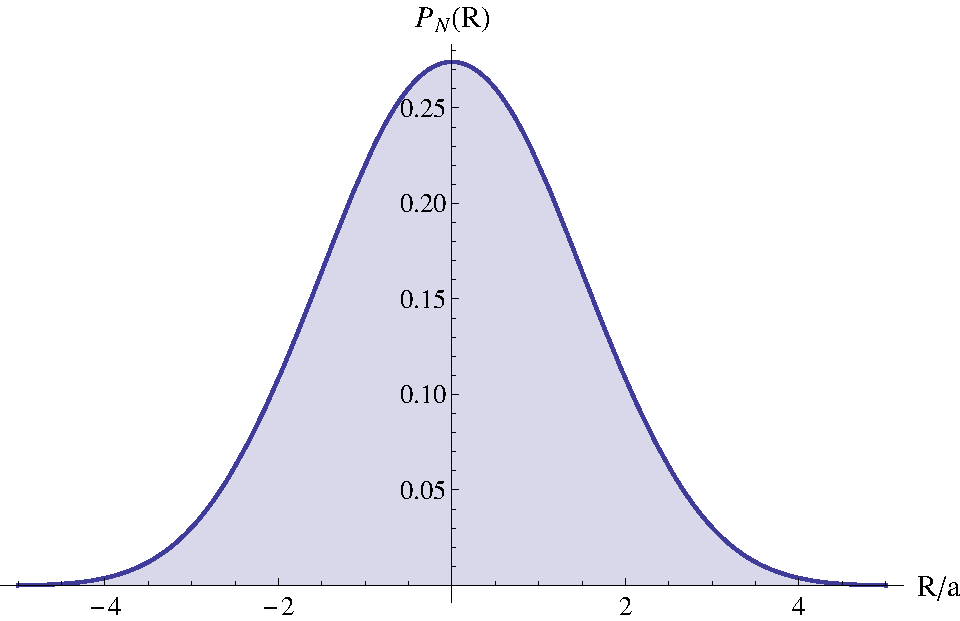
\includegraphics[scale=0.8]{Graphics/3D/PN_finitep05_N5.pdf}
\caption{A plot of the probability distribution of a EFJC ending at a position $R/a$ for $N=5$.}
\end{figure}
\end{comment}

\section{Conclusion}

Using the Fourier Transform Integral method we have presented a model which gives a partition function to describe an Extendable Freely Jointed Chain as an improvement to the non-extendable Freely Jointed Chain. The EFJC improves the standard FJC polymer model by allowing each link in the chain to extend and contract independently to emulate the mechanical behaviour of intermolecular bonds within polymers. 

In one dimension, the partition function for EFJC was calculated using two top-hat functions as the weighting function in the Fourier Transform integral. This potential allowed each link to move freely in one dimension that included a weighting function to provide linear extensibility. Taking a small approximation of $p$ in the EFJC model transformed the partition function to that of a FJC which was calculated using delta functions as the weighting functions. 

In \figref{Comparison3D} we see a plot which compares the results of $Z_{q}$ with N=4 for the FJC and the EFJC with different $p$. It is interesting to note that for extensions where the range of $p$ is less than $0.2a$ the results are almost identical. Above this range we see that the partition function distribution becomes larger in the EFJC model. 

With the negligible differences in the partition function distributions for small $p$ we can conclude that results from the EFJC can be well represented by those from the FJC.

%However, the EFJC holds true where the elasticity is linear, so determining the range of $p$ at which the behaviour stays linear would need to be taken into account as results for $p$ larger than $0.2a$ begin to differ significantly. 

%Extending this work further where more complex strutuces of polymers are involved, a more powerful and general method such as the Transfer Integral method will be used to calculate the partition function. The structure we will be focusing on is the collagen polymer which is a triple helix structure with hydrogen bonds between three component strands.
 

